\chapter{Results}
\section{VEGA reproducibility}\label{results:reproducibility}
\subsection{Reproducing results in VEGA paper}
Firstly, to verify the ability and availability of VEGA\cite{Seninge2021}, we reproduced the analyses of the published PBMCs (peripheral blood mononuclear cells) dataset\cite{Kang2018} which consists of two groups of blood cells: Control cells and cells stimulated with interferon-$\beta$ (see Methods \ref{methods:data}). We wanted to see whether VEGA could recapitulate biological information in its interpretable latent space using the Reactome collection of pathways and processes\cite{Jassal2020} as prior knowledge to initiate the wiring of the decoder part of VEGA (see Methods \ref{methods:prior}). The hyperparameters used in this section are recorded in Appendix \ref{appendixA}. After the model training, we ran UMAP\cite{McInnes2020} on the VEGA embedding (see Methods \ref{methods:umap}). The results show that VEGA was capable of clustering cells into cell types and treatment conditions (Fig.\ref{fig:reproducibility}A;Appx.\ref{fig:reproducibility_appx}). Moreover, when specifically looking into GMV activities, we observed that the GMV representing the interferon-$\alpha$/$\beta$ signaling pathway separated stimulated and control cells, which is consistent with our result and previous studies\cite{Mazewski2020} (Fig.\ref{fig:reproducibility}B).

Next, we wanted to see if the differential GMV activities between two treatment conditions are statistically significant. For this, we performed differential activity analysis proposed by Seninge et al. (2021). Since each GMV is modeled into the posterior distribution, two mutually exclusive hypotheses can be formulated (i.e., a given GMV activity is higher in the stimulated group compared to the control group or the other way around) and the posterior probabilities of these hypotheses can be approximated through Monte Carlo sampling from the GMV distributions. Finally, a Bayes factor\cite{Kass1995,Held2018} (BF), the ratio of the hypothesis probabilities, can be used to determine the significantly differential GMV activities between two treatment conditions (see Methods \ref{methods:bf}). The volcano plot indicates that the activities of interest (interferon-$\alpha$/$\beta$ signaling and interferon signaling pathways) were significantly more active in the stimulated cells compared to the control cells ($|\textnormal{log}_e(\textnormal{BF})|>3$, Fig.\ref{fig:reproducibility}C). Together, these reproduced results confirm the interpretability of VEGA, enabling us to interpret gene expression data from the view of biological pathways and processes.\vspace{7mm}

\begin{figure}[h!]
    \centering
    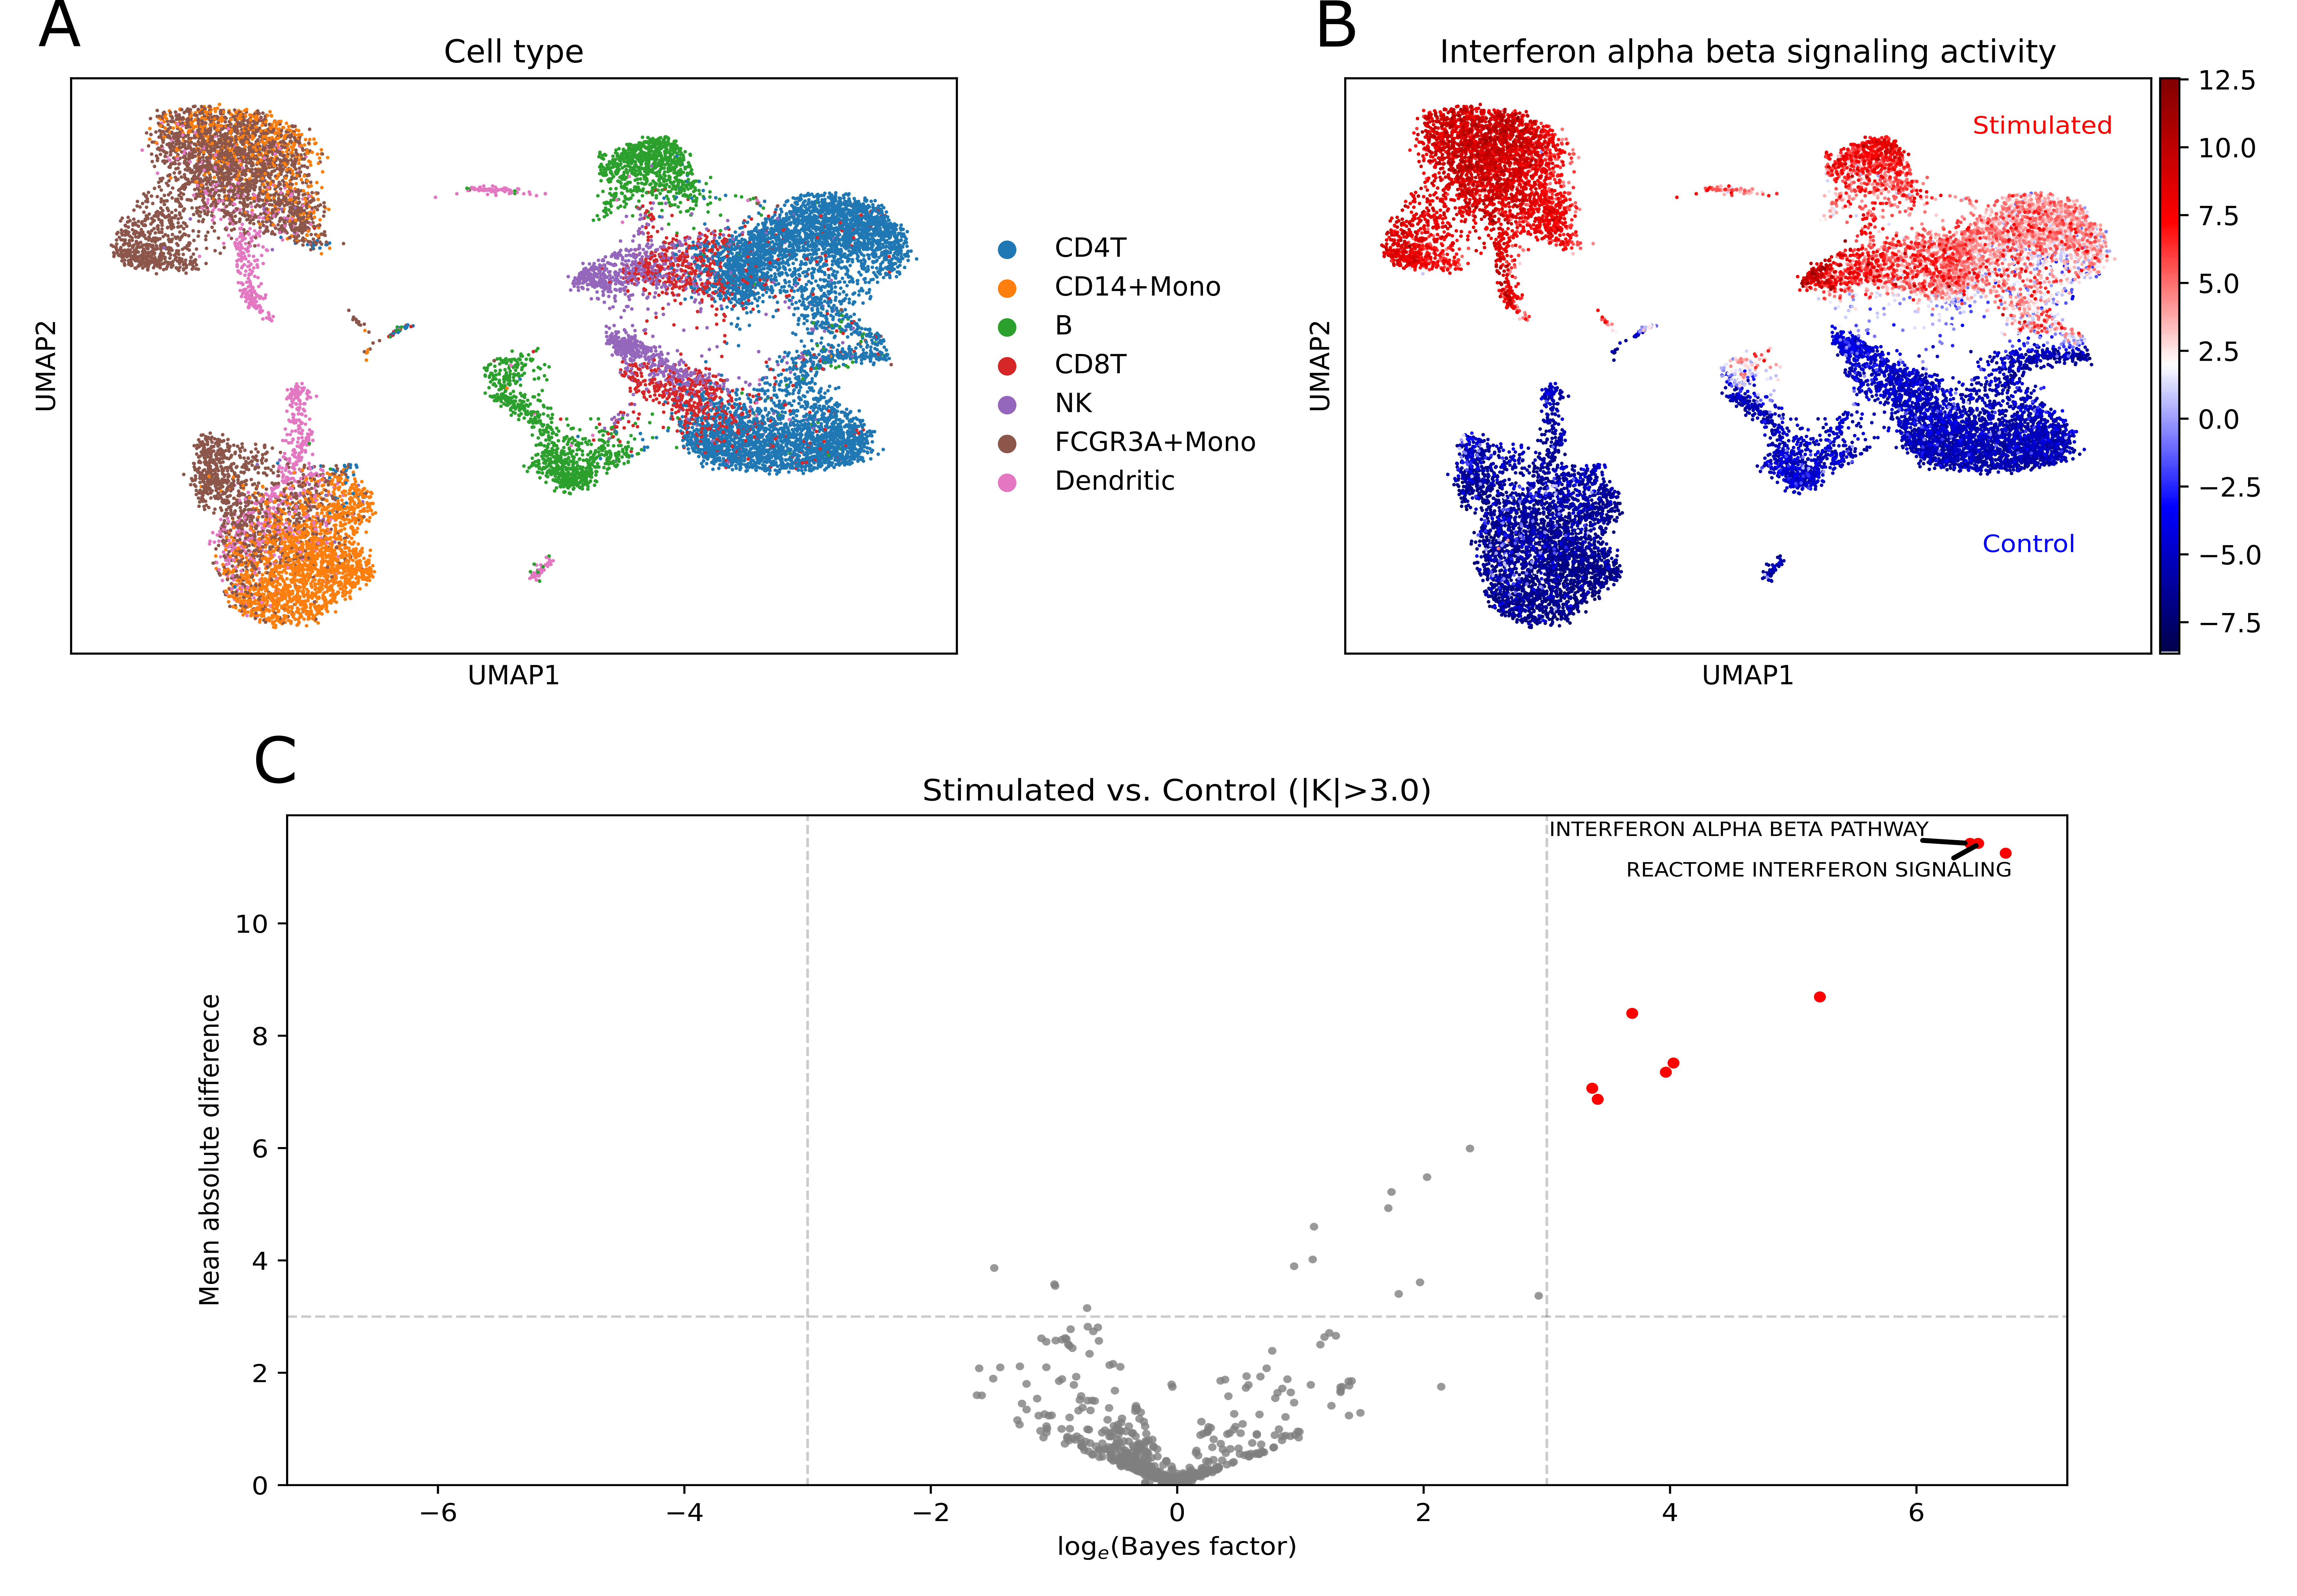
\includegraphics[scale=0.47]{reproducibility/reproducibility.png}
    \caption{\small{\textbf{Reproduction of results in VEGA paper} | We reproduced the PBMCs analysis using the Reactome pathways as the prior. \textbf{(A)} The UMAP plot shows the model could cluster cells into cell types. \textbf{(B)} Since the dataset consists of control cells and cells stimulated by interferon-$\beta$, the interferon-$\alpha$/$\beta$ signaling pathway was of interest. The UMAP plot colored by activity levels of the GMV representing the interferon-$\alpha$/$\beta$ signaling pathway shows that stimulated and control cells were nicely separated and the stimulated cell group had a high level of the activity. \textbf{(C)} The x-axis and the y-axis indicate the significance level and the mean absolute difference of activity comparisons between two cell types. The volcano plot shows that interferon-$\alpha$/$\beta$ signaling and interferon signaling pathways were significantly more active in stimulated cells. We considered pathways to be significantly differentially activated if $|\textnormal{log}_e(\textnormal{BF})|>3$.}}
    \label{fig:reproducibility}
\end{figure}

\subsection{Using dropout layer in latent space stabilizes model reproducibility}\label{sec:reproducibility}
At the beginning of this work, we performed benchmarks for VEGA in an attempt to check the interpretability of the model and understand how exactly the model works. Specifically, we were interested in the stability of VEGA training since we found that some of the GMV activities in the latent space could be unrelated or even anticorrelated between two individual trained models on the same dataset (see Methods \ref{methods:stability}). Take the PBMCs dataset\cite{Kang2018} as an example using the same hyperparameters specified above (see Appendix \ref{appendixA}). We observed that the median of the correlations between two matching GMVs was 0.75 and some of them had negative correlations (Fig.\ref{fig:stability}A). We wondered if there are hyperparameters in control of the reproducibility of the GMV activities and then first dissected this question by investigating two novel hyperparameters introduced in VEGA: A dropout layer and additional fully connected nodes in the latent space. Note that the model used as the control was with $z\_dropout=0.5$ and $add\_nodes=1$ and we tuned one of these two hyperparameters each time to see the changes in the reproducibility. We found that, without employing a dropout layer in the latent space ($z\_dropout=0$), the median of the correlations dropped to 0.42 and the anticorrelated events became even worse (up to $-0.8$, Fig.\ref{fig:stability}A). There was no notable difference in the model reproducibility using a dropout rate of 0.3 and 0.5. On the other hand, we observed that with or without using additional nodes in the latent space did not significantly affect the reproducibility, where the median of the correlations slightly decreased from 0.72 to around 0.65 (Fig.\ref{fig:stability}A). Collectively, we suggest that the implementation of a dropout layer in the latent space have the effect of stabilizing the model reproducibility.

We next questioned whether the correlation coefficients of matching GMVs have any relationships with the numbers of genes in the output layer they connect to. We calculated the number of genes connected to each GMV and vice versa according to the Reactome prior knowledge and the considered highly variable genes (Appx.\ref{fig:stability_appx}). We display the results of using $z\_dropout=0.5$ and 0 (both with $add\_nodes=1$) for this task because we observed that employing a dropout layer in the latent space is a way to improve the model training stability. The results do not show any evident correlations between the reproducibility of GMVs and the numbers of genes which GMVs connect to (Fig.\ref{fig:stability}B,C). However, interestingly, we observed that additional nodes in the latent space always had a high correlation coefficient (0.99) when there was only one additional node employed, but had varied correlation coefficients ranging from -0.76 to 0.99 when more than one additional nodes were used (Fig.\ref{fig:stability}D). We infer that these additional nodes randomly shared learnable information with each other in different individual trained models since they all fully connected to genes in the output layer, leading to the poor characterization. Therefore, when we computed correlations, two corresponding latent variables might hold different information, leading to a low correlation coefficient. To this end, we propose the possible further work could be the investigation of whether gene programs having highly similar gene sets in prior information used to initiate the decoder wiring blur the reproducibility and the interpretability of GMVs because VEGA fails to model certain latent variables to specific biologically meaningful gene programs.\vspace{17mm}

\begin{figure}[h!]
    \centering
    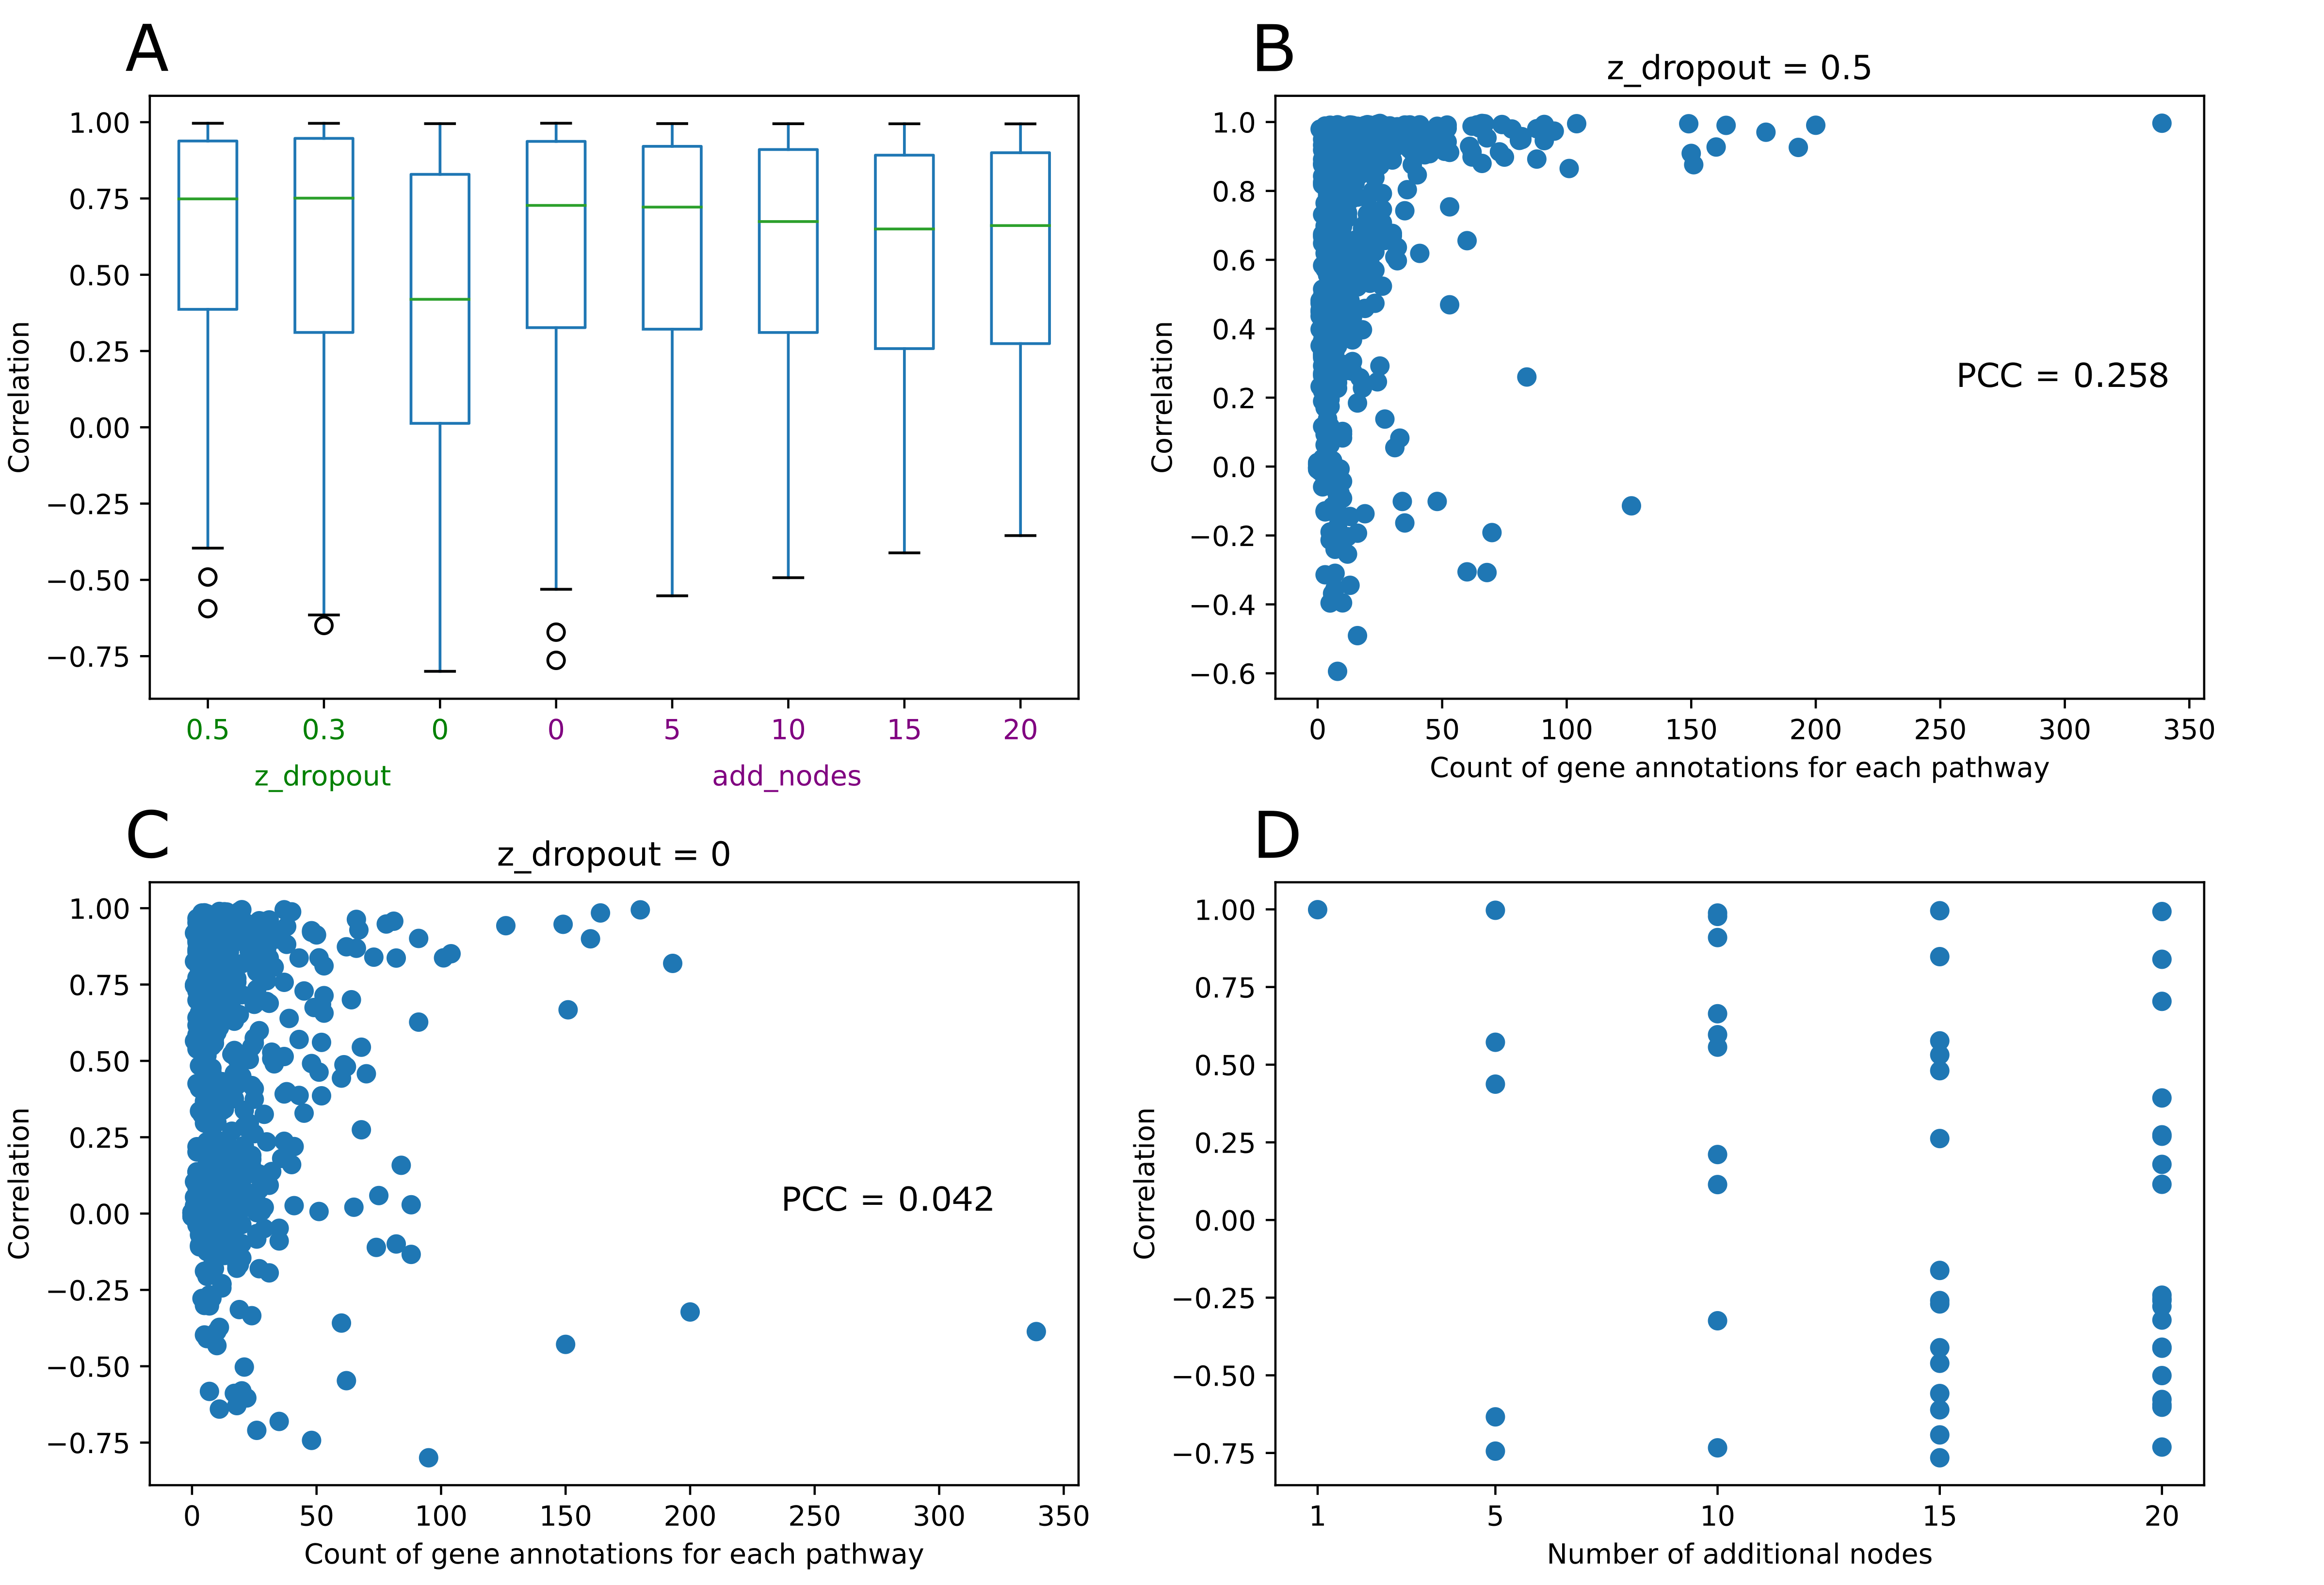
\includegraphics[scale=0.70]{reproducibility/stability.png}
    \caption{\small{The caption is on the next page.}}
    \label{fig:stability}
\end{figure}

\newpage

\addtocounter{figure}{-1}
\begin{figure}[t!]
    \caption{\small{\textbf{Investigation of model training stability} | The method we used to measure the model training stability was computing Pearson correlation coefficients between two matching GMVs from two individual trained models using the same set of hyperparameters. We tuned two hyperparameters used in the latent space, one at a time: (1) \textit{z\_dropout} (the dropout rate) and \textit{add\_nodes} (the number of additional fully connected nodes) to investigate the changes in the training stability. Note that the correlations of the additional fully connected nodes were excluded from plot A, B and C. \textbf{(A)} The x-axis indicates the value of a hyperparameter and the y-axis indicates the correlation coefficient. The first boxplot ($z\_dropout=0.5$ and $add\_nodes=1$) was used as the control. The boxplots show that using a dropout layer in the latent space improved the stability of model training (green) and the number of additional nodes used in the latent space did not have influence on the training stability (purple). The box extends from the Q1 (25$\textsuperscript{th}$ percentile) to the Q3 (75$\textsuperscript{th}$ percentile) of data with the horizontal line inside denoting the median of data (Q2, 50$\textsuperscript{th}$ percentile). The whiskers extend from the box show the range of data (Q0, 0$\textsuperscript{th}$ percentile and Q4, 100$\textsuperscript{th}$ percentile) if all data points are within 1.5 * IQR (IQR = Q3 - Q1). Otherwise, the data points beyond the range are displayed as separate circles. IQR stands for interquartile range. \textbf{(B,C)} The x-axis indicates the number of genes each GMV connects to. The scatterplots show there were no evident correlations between the reproducibility of GMVs and the numbers of genes which GMVs connect to. PCC stands for Pearson correlation coefficient. \textbf{(D)} The x-axis indicates the number of additional fully connected nodes used in the latent space. The plot shows the reproducibility of some additional nodes could be very unstable when the number of additional nodes used was more than 1. The reason may be that the additional nodes randomly shared the learned information due to the same decoder wiring.}}
\end{figure}

\section{Performing benchmarks for VEGA}\label{results:benchmarks}
\subsection{TF activity analysis recapitulates adrenal medulla development}\label{sec:sparse_adm}
Secondly, we applied VEGA\cite{Seninge2021} to the published human adrenal medulla dataset\cite{Jansky2021} which consists of Schwann cell precursors (SCPs), chromaffin cells, neuroblasts and the other transient cells in the adrenal medulla from various stages of embryonic and fetal development (see Methods \ref{methods:data}). The UMAP\cite{McInnes2020} embedding of the gene expression space of the adrenal medulla cells shows the nice cell clustering and developmental trajectories where SCPs gave rise to chromaffin cells and neuroblasts through bridge and connecting progenitor cells\cite{Jansky2021} (Fig.\ref{fig:sparse_adm_scenic}A, see Methods \ref{methods:umap}). Moreover, the UMAP plot colored by samples reveals that the cell clustering was subject to biological differences between the cell types rather than technical differences between the samples (Appx.\ref{fig:sparse_adm_scenic_appx}A). As mentioned previously, owing to the flexibility of the GMV specification, we employed the SCENIC\cite{Aibar2017} regulons inferred from this human adrenal medulla dataset\cite{Jansky2021} as prior biological knowledge to guide the decoder wiring (see Methods \ref{methods:prior}). We wanted to see how capable VEGA is to capture TF activities at the single-cell level in its latent space, which can be used to conduct cell clustering and differential activity analysis. We first split the task into three parts where VEGA models were trained on (1) the dataset with the top 2000 highly variable genes, (2) the dataset with the whole gene features and (3) the dataset with only those genes connected to the GMVs according to the SCENIC regulons. The hyperparameters used in this task are recorded in Appendix \ref{appendixA}. After the VEGA training, we ran UMAP on the VEGA embeddings. Among these three trained models, all of them could nicely cluster cells into cell types (Fig.\ref{fig:sparse_adm_scenic}B;Appx.\ref{fig:sparse_adm_scenic_appx}B,C). Even so, the model trained on the dataset with the top 2000 highly variable genes best preserved the adrenal medulla development, which was thereby mainly used for the further work.

To investigate whether these GMVs truly represented certain SCENIC regulons, we performed differential activity analysis to statistically compare GMV activities between different cell types (see Methods \ref{methods:bf}). Note that the inferred TF activities of each adrenal medulla cell type group described in Jansky et al. (2021) were used as references for our benchmarks (Fig.\ref{fig:sparse_adm_scenic}C). The volcano plots show that VEGA precisely modeled the latent variables as the corresponding TFs in the prior because nearly all of the GMV (TF) activities of interest, except HES6, were averagely active in correct cell type groups (Fig.\ref{fig:sparse_adm_scenic}D) according to the references in Fig.\ref{fig:sparse_adm_scenic}C. For example, GATA3 and TFAP2B were found to have a high level of activities in neuroblasts and many members of the JUN/FOS TF family are associated with the chromaffin differentiation\cite{Jansky2021}. In the light of the ability of VEGA, those TFs which had significantly differential activities between different cell types but were not captured in Jansky et al. (2021), such as SREBF2 and E2F1 in neuroblasts compared to SCPs (Appx.\ref{fig:sparse_adm_scenic_appx}D), are extremely worth further investigation. However, we did not find any supporting biological evidence from previous studies for them in the context of healthy cells. Therefore, further work on verifying whether those significantly differential TF activities are biologically meaningful or just false positives is needed. Last but not least, the one additional fully connected node we used in the latent space was significantly active in neuroblasts and in chromaffin cells compared to SCPs, which indicates employing additional nodes helps capture extra information that is not explained in the prior (UNANNOTATED\_0 in Appx.\ref{fig:sparse_adm_scenic_appx}D).

\newpage

\begin{figure}[H]
    \centering
    \hspace*{-2mm}
    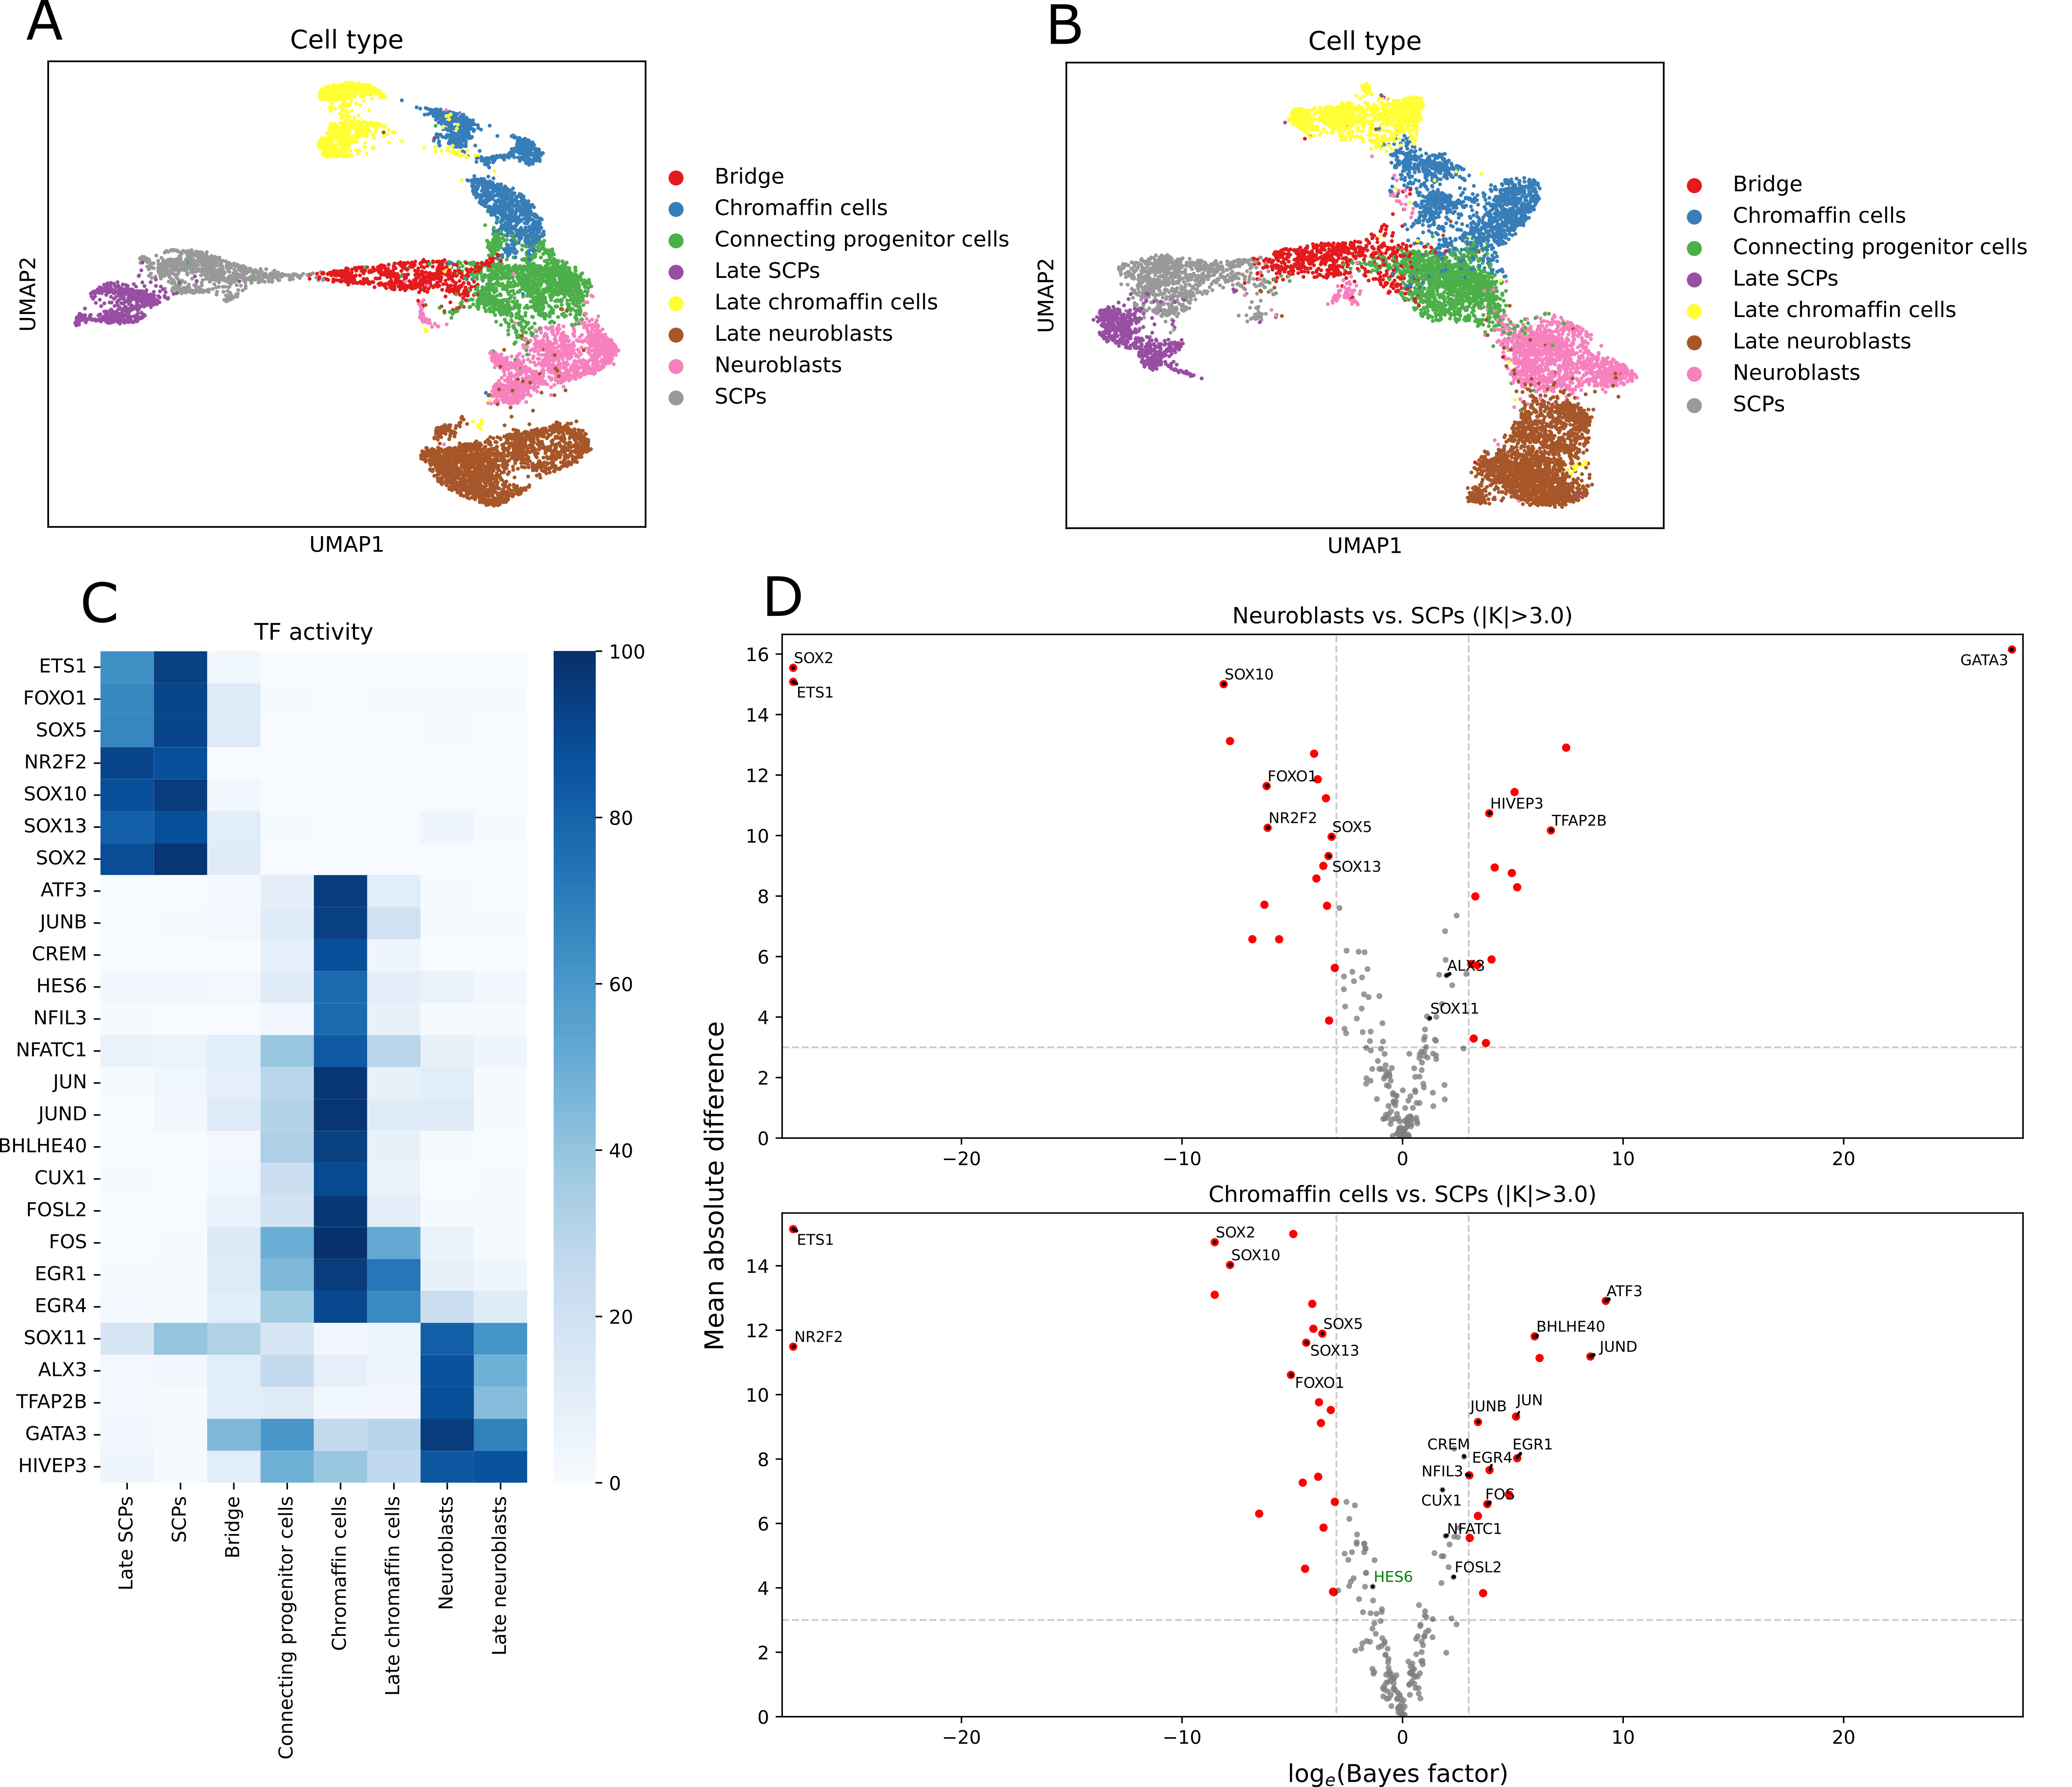
\includegraphics[scale=0.72]{SCENIC_sparse/adm_scenic_hvg_sparse.png}
    \caption{\small{\textbf{Benchmarks for VEGA} | We used the SCENIC regulons inferred from the human adrenal medulla dataset as prior knowledge to analyze TF activities of human adrenal medullary cells. \textbf{(A)} The UMAP embedding of the gene expression space shows the clear cell clustering and the developmental trajectories of the adrenal medulla. \textbf{(B)} The UMAP embedding of the VEGA latent space shows that the model could cluster cells into cell types and preserve the developmental trajectories. Note that the model were trained on the dataset with the top 2000 highly variable genes and we removed 23 SCENIC regulons from the prior, whose target genes did not overlap with any considered gene features, i.e., there would be no connections between these 23 GMVs and the genes in the output layer. \textbf{(C)} The inferred TF activities of each cell type group from Jansky et al. (2021) were used as references for our TF differential activity analysis. Firstly, the TF activities in individual cells were inferred using SCENIC and for each TF, the activities across cells were discretized into two levels (active or inactive) using k-means clustering. Finally, the TF activities of each cell type group were determined by computing the fraction of cells whose TF states were active in each cell type. \textbf{(D)} The x-axis and the y-axis indicate the significance level and the mean absolute difference of activity comparisons between two cell types. The volcano plots show that nearly all of the TF activities of interest, except HES6 (colored in green), were averagely active in correct cell type groups. We considered TFs to be significantly differentially activated if $|\textnormal{log}_e(\textnormal{BF})|>3$.}}
    \label{fig:sparse_adm_scenic}
\end{figure}

\newpage

\subsection{Hard-coded decoder leaves little freedom for further inferences}
Next, instead of using the dataset-specific prior to initiate the decoder wiring, we employed the DoRothEA\cite{Garcia-Alonso2019} regulons which is not context-specific to investigate the behavior of VEGA (see Methods \ref{methods:prior}). Of note, the hyperparameters used in this task are the same as Section \ref{sec:sparse_adm}, which is recorded in Appendix \ref{appendixA}. After the model training, we ran UMAP on the VEGA embedding. The result shows that VEGA was still able to cluster cells into cell types and also exhibit the developmental trajectories of the human adrenal medulla (Fig.\ref{fig:sparse_adm_dorothea_hvg}A). However, when we looked into the differential activity analysis results, we observed that VEGA using the general prior knowledge could not faithfully reflect the correct activations of TF activities in certain cell types anymore (Fig.\ref{fig:sparse_adm_dorothea_hvg}B). The differential activity analysis results took Fig.\ref{fig:sparse_adm_scenic}C as references. Although nearly all of the significantly differential TF activities, except CUX1, were correctly presented in the corresponding cell types, a majority of TF activities could not be captured or were even falsely predicted by VEGA (e.g., HIVEP3, JUNB, JUND and so on). We then checked the overlaps of the target genes between the DoRothEA and the SCENIC regulons and found that all target gene sets hardly overlap with each other (Table \ref{table:dorothea_scenic_outline}). Collectively, these results indicate that VEGA has limited freedom to further make inferences beyond the prior and fails to provide the interpretability in the latent space when prior knowledge used is not context-specific. Given that we still obtained such the clear clustering of the adrenal medullary cells, we reasoned that the compressed information that the VEGA latent variables hold can be extracted from the expression data with any decoder settings, but just the learned information will be randomly distributed in the latent space if the decoder wiring is biologically meaningless, which means the model loses its interpretability. This hypothesis will be corroborated in the next section.

\newpage

\begin{figure}[h!]
    \centering
    \hspace*{-5mm}
    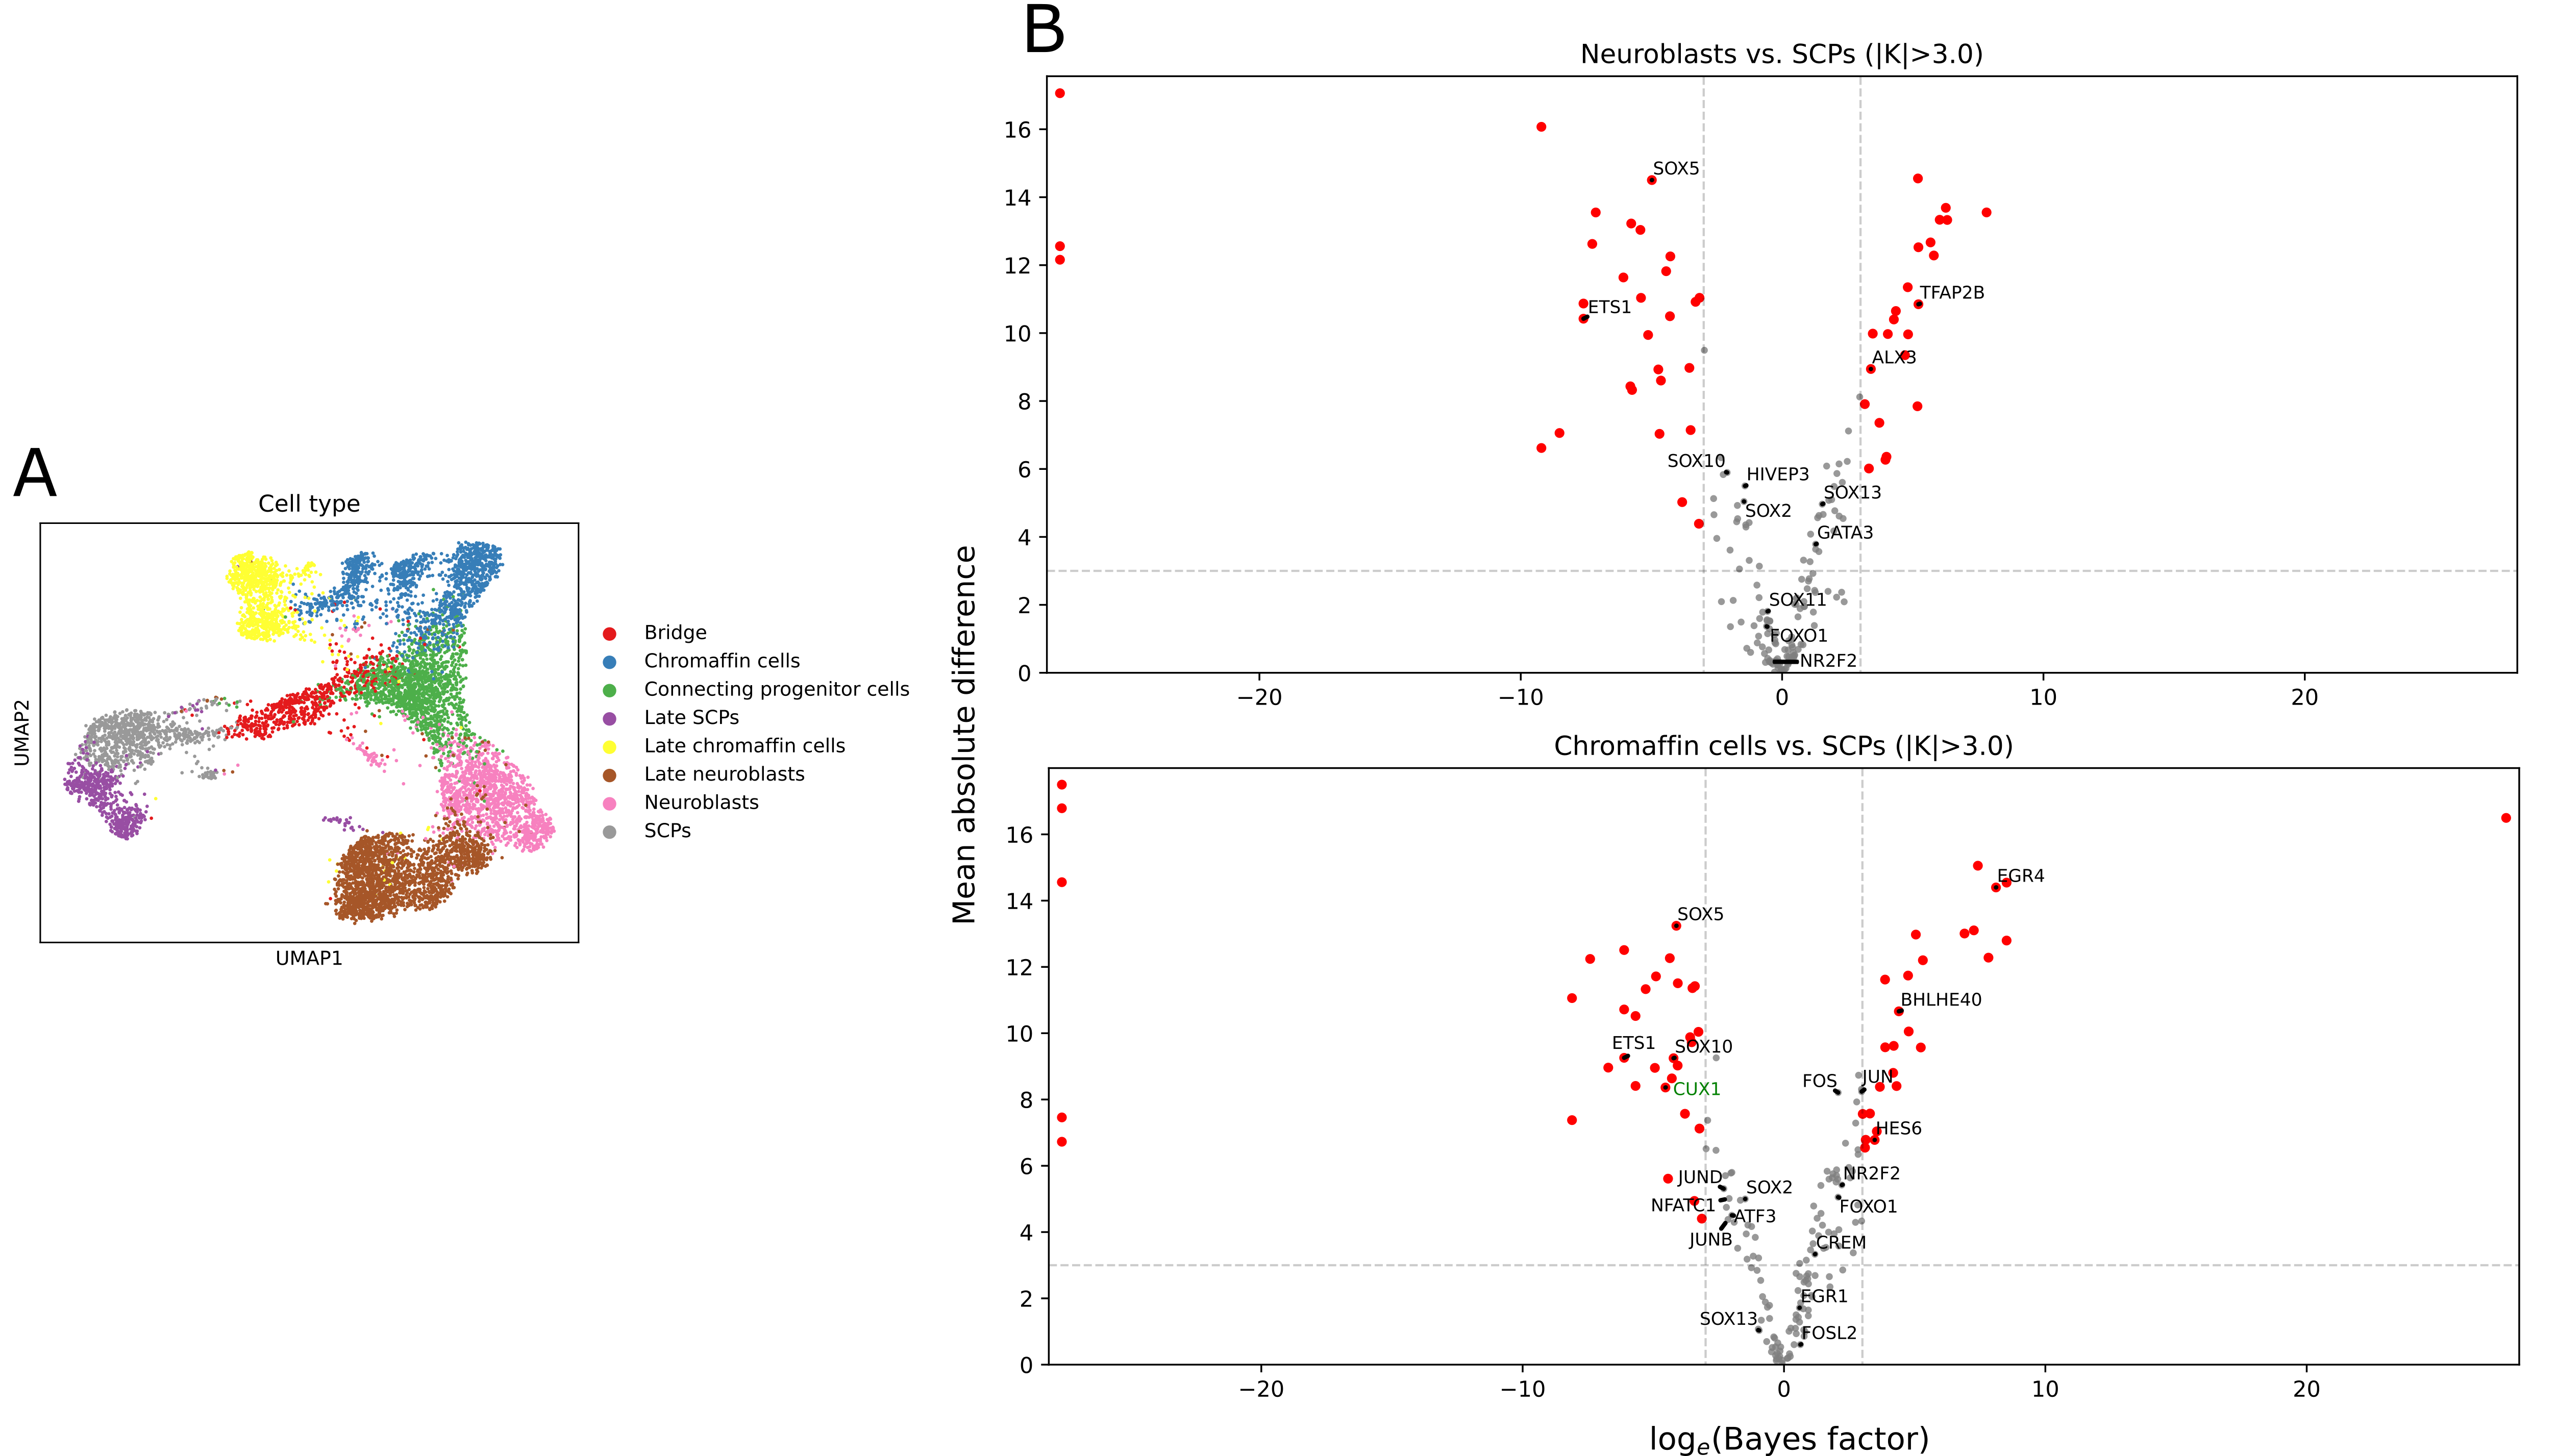
\includegraphics[scale=0.76]{DoRothEA_sparse/adm_dorothea_hvg.png}
    \caption{\small{\textbf{Observations of VEGA using general regulons as prior knowledge} | We used the DoRothEA regulons which is not context-specific as the prior to investigate the changes in the model interpretability. \textbf{(A)} The UMAP plot shows the model could still cluster cells into cell types and preserve the developmental trajectories of the adrenal medulla. Note that we removed 19 DoRothEA regulons from the prior, whose target genes did not overlap with any considered gene features. \textbf{(B)} The x-axis and the y-axis indicate the significance level and the mean absolute difference of activity comparisons between two cell types. Note that the differential activity analysis results took Fig.\ref{fig:sparse_adm_scenic}C as references. The volcano plots show that even though nearly all the significantly differential TF activities, except CUX1 (colored in green), were correctly predicted, a majority of TF activities could not be captured or were even wrongly predicted (e.g., HIVEP3, JUNB and JUND) by the model. We considered TFs to be significantly differentially activated if $|\textnormal{log}_e(\textnormal{BF})|>3$.}}
    \label{fig:sparse_adm_dorothea_hvg}
\end{figure}

\begin{table}[h!]
    \begin{center}
        \captionsetup{width=.77\textwidth}
        \caption{\small{\textbf{Outline of DoRothEA and SCENIC regulons of interest} | Confidence levels are of DoRothEA, ranging from A (most confident) to E (least confident) depending on the amount of supporting biological evidence.}}
        \label{table:dorothea_scenic_outline}
        \begin{tabular}{|c|c|c|c|c|c|}
        \hline
        & \textbf{\small{Confidence}} & \textbf{\small{Gene set size}} & & \textbf{\small{Overlapping of}}\\
        \textbf{\small{TF}} & \textbf{\small{level}} & \textbf{\small{-DoRothEA-}} & \textbf{\small{-SCENIC-}} & \textbf{\small{target genes}}\\
        \hline
        \small{ALX3} & \small{E} & \small{385} & \small{101} & \small{4}\\
        \hline
        \small{ATF3} & \small{C} & \small{50} & \small{970} & \small{8}\\
        \hline
        \small{BHLHE40} & \small{C} & \small{58} & \small{633} & \small{5}\\
        \hline
        \small{CREM} & \small{C} & \small{52} & \small{1715} & \small{24}\\
        \hline
        \small{CUX1} & \small{C} & \small{41} & \small{617} & \small{5}\\
        \hline
        \small{EGR1} & \small{A} & \small{124} & \small{299} & \small{5}\\
        \hline
        \small{EGR4} & \small{E} & \small{476} & \small{62} & \small{4}\\
        \hline
        \small{ETS1} & \small{A} & \small{145} & \small{868} & \small{6}\\
        \hline
        \small{FOS} & \small{A} & \small{90} & \small{1071} & \small{10}\\
        \hline
        \small{FOSL2} & \small{A} & \small{10} & \small{1557} & \small{1}\\
        \hline
        \small{FOXO1} & \small{A} & \small{43} & \small{396} & \small{4}\\
        \hline
        \small{GATA3} & \small{A} & \small{73} & \small{543} & \small{1}\\
        \hline
        \small{HES6} & \small{E} & \small{199} & \small{202} & \small{4}\\
        \hline
        \small{HIVEP3} & \small{E} & \small{192} & \small{13} & \small{0}\\
        \hline
        \small{JUN} & \small{A} & \small{121} & \small{1975} & \small{19}\\
        \hline
        \small{JUNB} & \small{C} & \small{52} & \small{673} & \small{3}\\
        \hline
        \small{JUND} & \small{A} & \small{19} & \small{3470} & \small{3}\\
        \hline
        \small{NFATC1} & \small{C} & \small{35} & \small{120} & \small{0}\\
        \hline
        \small{NFIL3} & \small{D} & \small{11} & \small{252} & \small{0}\\
        \hline
        \small{NR2F2} & \small{A} & \small{18} & \small{287} & \small{0}\\
        \hline
        \small{SOX10} & \small{A} & \small{16} & \small{285} & \small{3}\\
        \hline
        \small{SIX11} & \small{C} & \small{29} & \small{161} & \small{1}\\
        \hline
        \small{SOX13} & \small{C} & \small{42} & \small{14} & \small{0}\\
        \hline
        \small{SOX2} & \small{A} & \small{10} & \small{168} & \small{0}\\
        \hline
        \small{SOX5} & \small{E} & \small{875} & \small{160} & \small{29}\\
        \hline
        \small{TFAP2B} & \small{E} & \small{796} & \small{984} & \small{55}\\
        \hline
        \end{tabular}
    \end{center}
\end{table}

\subsection{Randomizing predefined gene sets breaks model interpretability}
To scrutinize the importance of prior biological knowledge in terms of the interpretability of the VEGA latent space, we randomized the aforementioned SCENIC regulons inferred from the human adrenal medulla dataset\cite{Jansky2021} on varied levels (from 10\% to 90\%) and trained VEGA using them as the prior to see the changes in the interpretability (see Methods \ref{methods:randomization}). Of note, the set of hyperparameters used in this task is the same as Section \ref{sec:sparse_adm}, which is recorded in Appendix \ref{appendixA}. The UMAP embeddings of the latent spaces show that the models could cluster cells into cell types and retain the developmental trajectories no matter how randomized the \textit{a priori} defined gene sets were (Fig.\ref{fig:sparse_adm_rand_hvg}A). This result is theoretically expected because the compressed information that the VEGA latent variables hold mainly depends on the encoder part. The latent variables should in principle be able to learn the learnable variation in the gene expression data with any decoder settings. However, randomizing the predefined gene sets affected the VEGA interpretability to different degrees depending on the level of randomization. The models could preserve the interpretability when slightly randomized gene sets (up to 30\%) were used as the prior, which indicates little incorrect information in prior knowledge is tolerable (Fig.\ref{fig:sparse_adm_rand_hvg2};Appx.\ref{fig:sparse_adm_rand_hvg_appx}). From 40\% randomization, the models started making some obvious mistakes. For example, SOX11 has been found having high TF activities in neuroblasts, many members of the JUN TF family are associated with the chromaffin differentiation and FOXO1 has higher TF activities in SCPs compared to neuroblasts\cite{Jansky2021} (Fig.\ref{fig:sparse_adm_rand_hvg2};Appx.\ref{fig:sparse_adm_rand_hvg_appx}). These previous findings could not be presented by the corresponding GMVs for differential activity tests when the prior knowledge was greatly disorganized. Finally, when 90\% of target genes in the prior were shuffled, most of the GMVs could not faithfully reflect differential TF activities in different cell types anymore (Fig.\ref{fig:sparse_adm_rand_hvg2}). Of note, the differential activity analysis results took Fig.\ref{fig:sparse_adm_scenic}C as references.

Furthermore, we looked into the learning curves of VEGA which used these different levels of randomized gene sets as prior knowledge. We observed that the efficiency of the model training was highly related to the correctness of the prior knowledge, where the training loss dropped more rapidly when less randomized predefined gene sets were provided (Fig.\ref{fig:sparse_adm_rand_hvg}B). To be more concretely, simulating the decoder wiring as real gene regulatory networks (GRNs) helps VEGA discern relationships between TFs and genes, resulting in more efficient learning. For predictive performance, the validation loss reveals that the models trained using the original and up to 20\% randomized gene sets outperformed the other models trained using more than 20\% randomized gene sets and there was no apparent difference among the original prior, 10\% and 20\% randomized gene sets, which implies VEGA should be able to tolerate a bit of wrong information in the prior knowledge (Fig.\ref{fig:sparse_adm_rand_hvg}C). This finding is in line with our earlier differential activity test results, showing the models' interpretability could be preserved when the gene sets were mildly randomized (Fig.\ref{fig:sparse_adm_rand_hvg2}). To sum up, correct prior knowledge is important for VEGA to keep the interpretability and generate accurate inferences. Slightly wrong prior knowledge is acceptable but when the prior is incorrect to the certain degree, VEGA starts losing its interpretability since the hard-coded linear decoder leaves no room for correcting prior knowledge\cite{Seninge2021}.

\newpage

\begin{figure}[H]
    \centering
    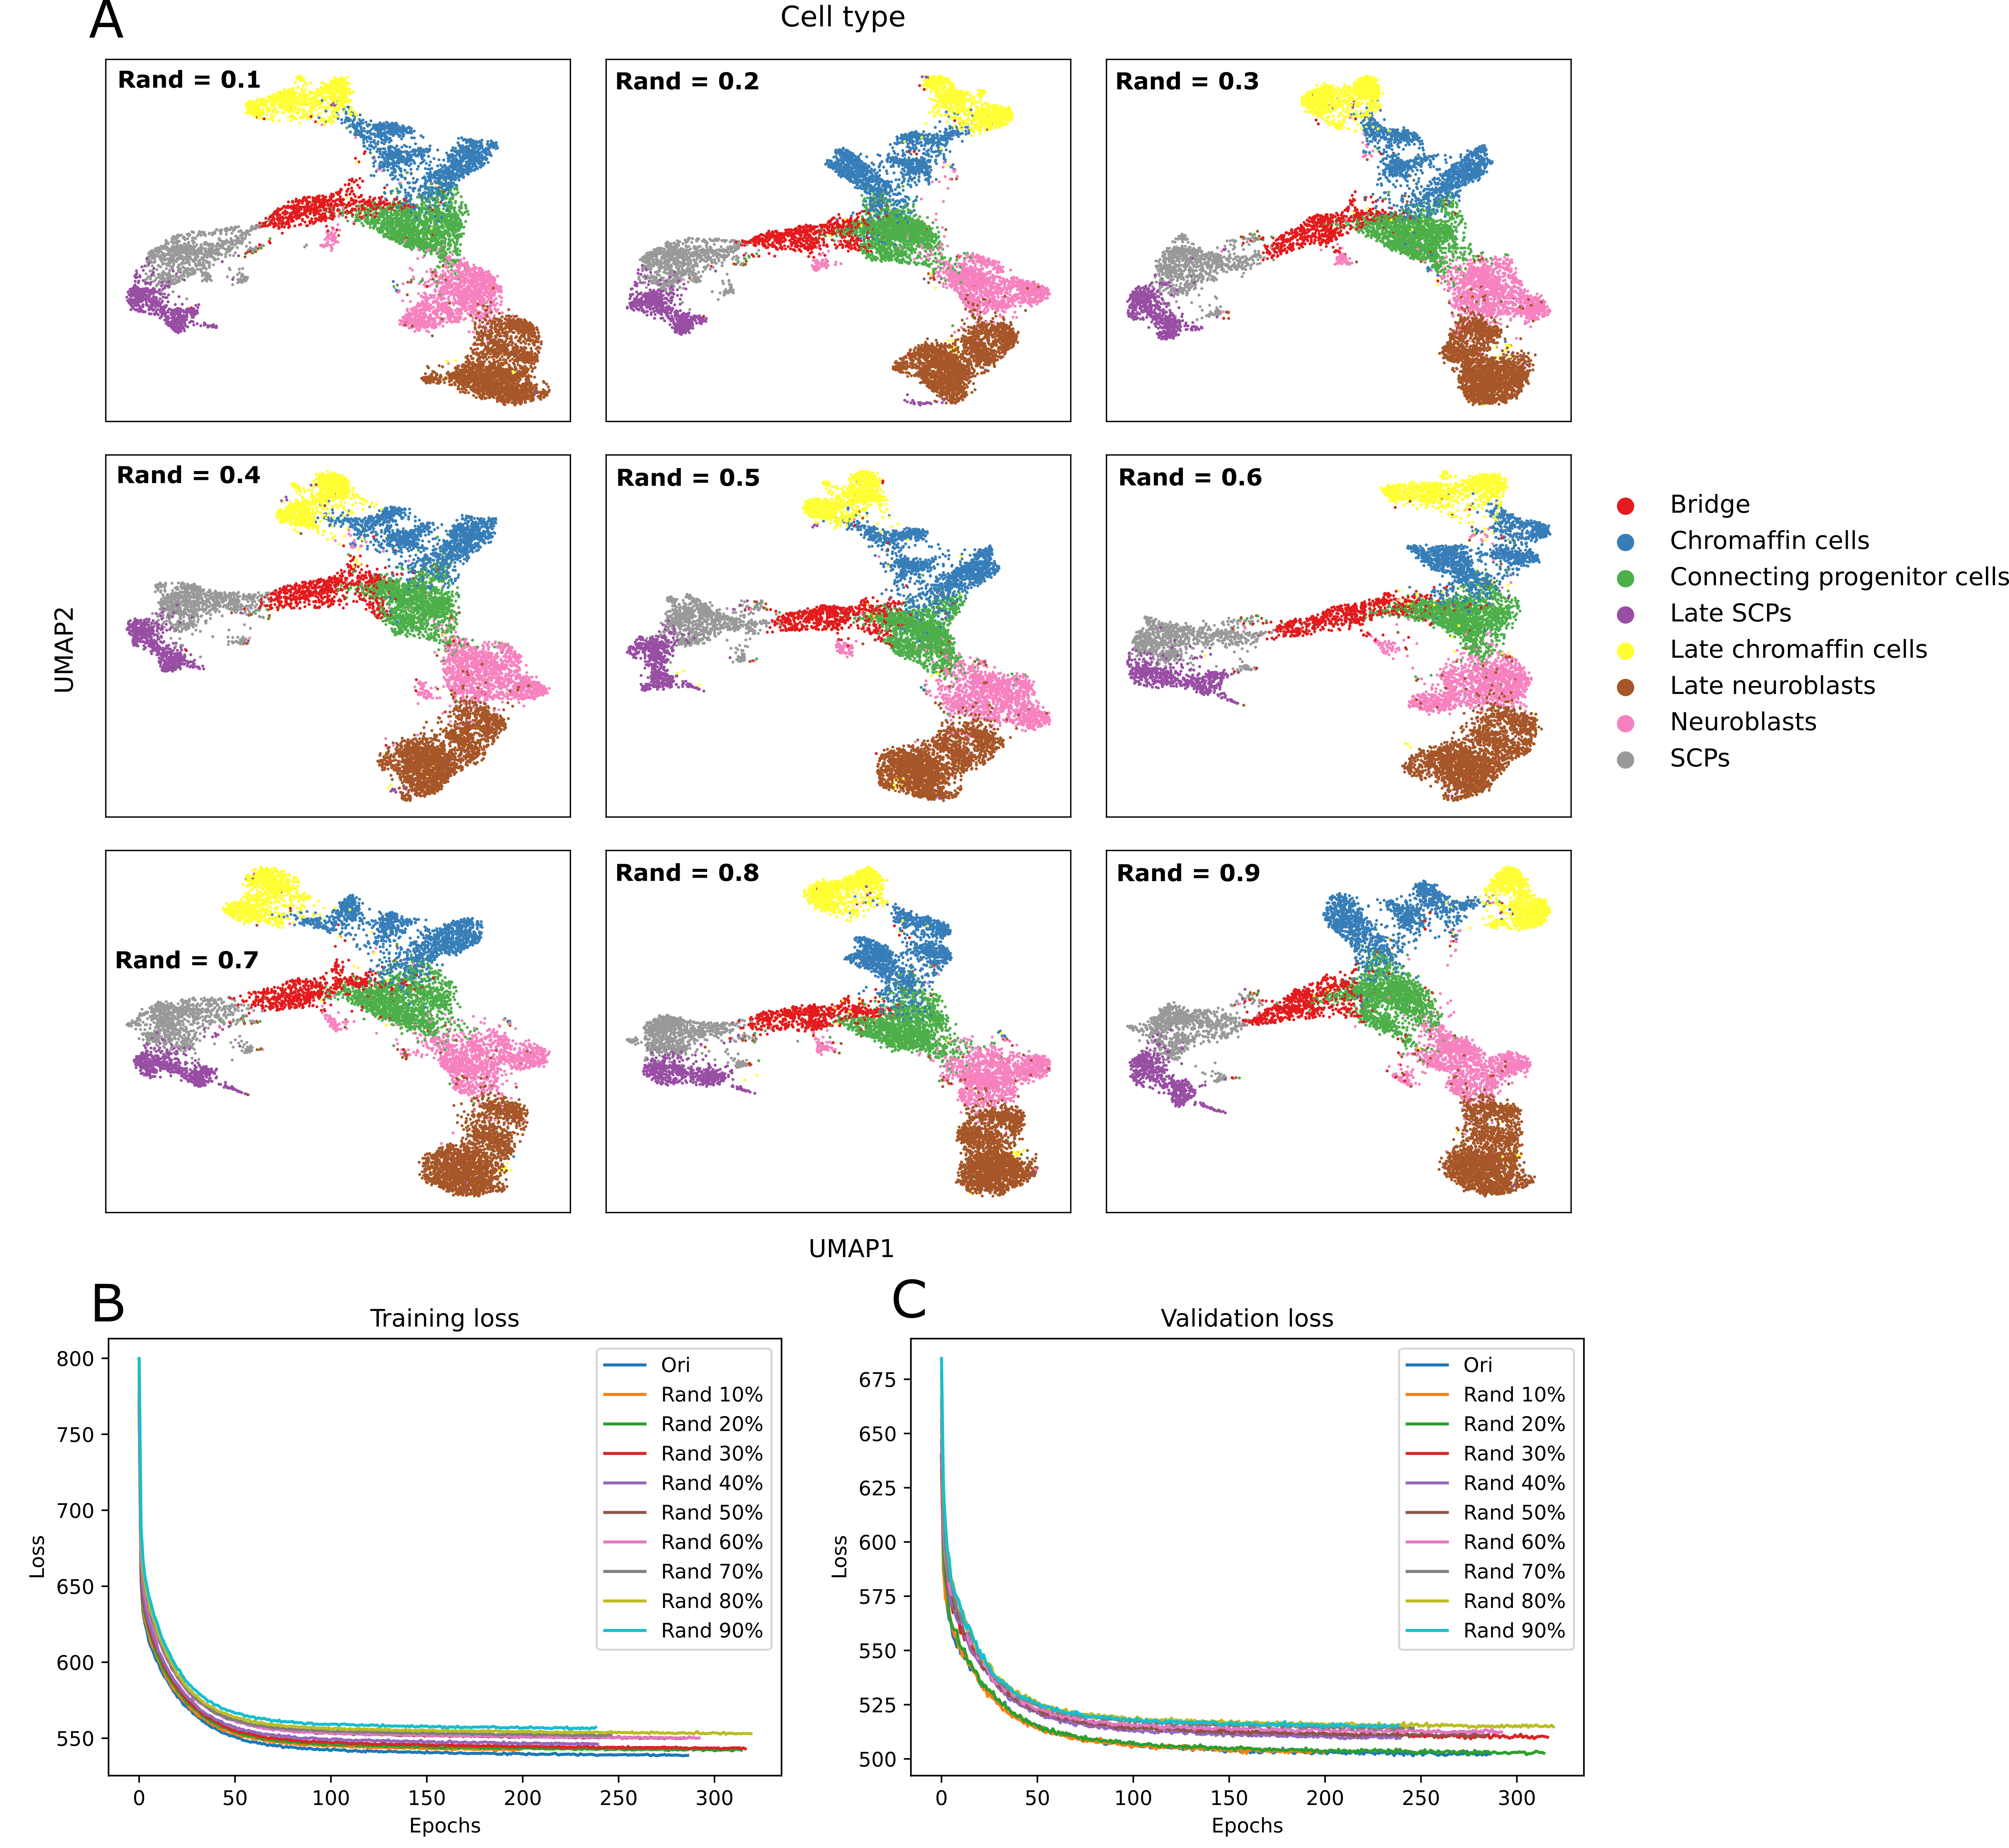
\includegraphics[scale=0.72]{SCENIC_sparse/adm_rand_hvg.png}
    \caption{\small{\textbf{Investigation of model behavior by using disorganized prior} | We randomized the SCENIC regulons inferred from the human adrenal medulla data to different degrees (10\% - 90\%) to investigate the changes in the model behavior. \textbf{(A)} The UMAP plots show that the models could cluster cells into cell types and preserve the adrenal medulla developmental trajectories no matter how randomized the prior was, which corroborates VEGA is able to learn variation in gene expression data with any decoder settings. Note that we removed the same 23 SCENIC regulons from the prior, whose target genes did not overlap with any considered gene features from all versions of the prior knowledge. Rand indicates the degree of randomization of the prior. \textbf{(B,C)} The x-axis indicates the epoch of model training and the y-axis indicates the training and the validation loss. The loss curves show that the training efficiency was highly related to the correctness of the prior (see plot B) and the model could tolerate little wrong information in the prior (up to 20\% randomization, see plot C). Ori represents the original prior and Rand represents the randomized prior to different degrees.}}
    \label{fig:sparse_adm_rand_hvg}
\end{figure}

\newpage

\begin{figure}[H]
    \centering
    \hspace*{-10mm}
    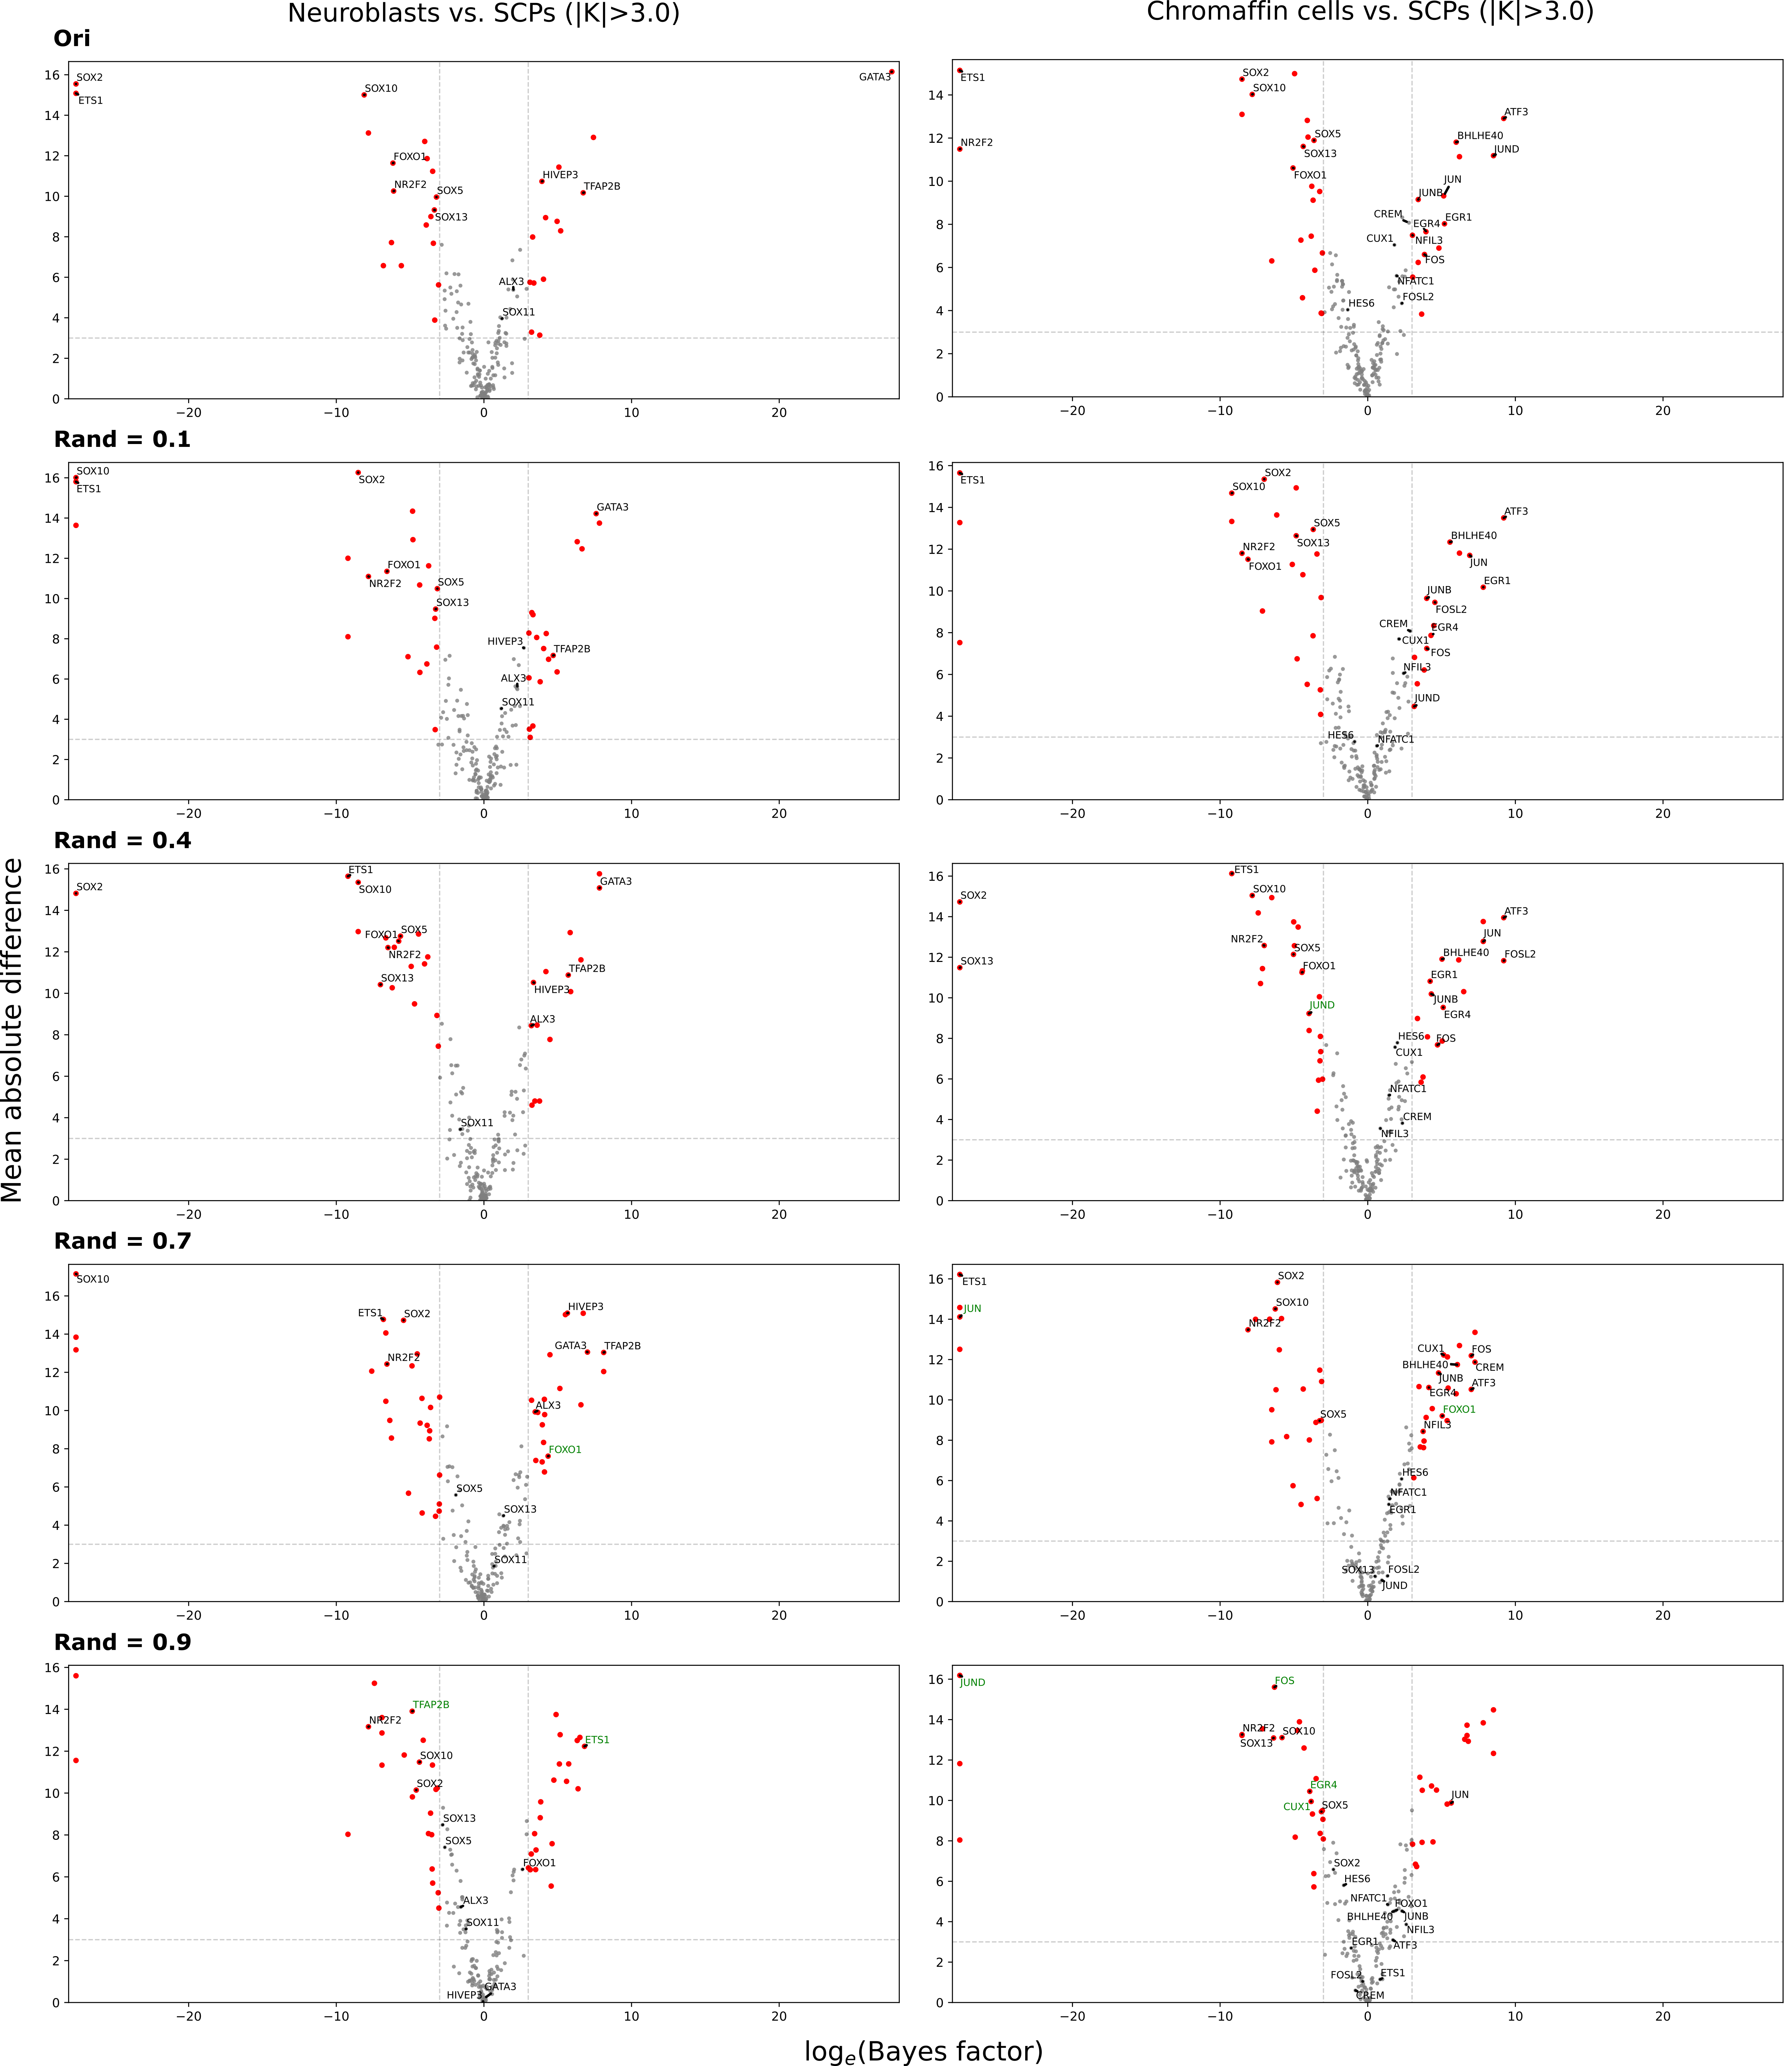
\includegraphics[scale=0.8]{SCENIC_sparse/adm_rand_hvg2.png}
    \caption{\small{The caption is on the next page.}}
    \label{fig:sparse_adm_rand_hvg2}
\end{figure}

\addtocounter{figure}{-1}
\begin{figure}[h!]
    \caption{\small{\textbf{Changes in model interpretability when randomizing prior to different degrees} | The x-axis and the y-axis indicate the significance level and the mean absolute difference of GMV activity comparisons between two cell types. Note that the differential activity analysis results took Fig.\ref{fig:sparse_adm_scenic}C as references. The volcano plots show that the model kept the interpretability when the prior was 10\% randomized, made some obvious mistakes (TFs colored in green) when the prior was 40\% and 70\% randomized and failed to capture most of the TFs of interest when the prior was 90\% randomized. Rand indicates the degree of randomization of the prior. We considered TFs to be significantly differentially activated if $|\textnormal{log}_e(\textnormal{BF})|>3$.}}
\end{figure}

\subsection{Incorporating batch annotations in model combats batch effects}
Deep generative models taking batch information into account have been demonstrated to have the ability to combat batch effects which frequently occur in single-cell transcriptome measurements\cite{Lopez2018}. VEGA, as an interpretable VAE, can take advantage of this technique and incorporate batch annotations in the encoder and the latent space (see Methods \ref{methods:model}). To test the function of batch correction of VEGA, we used the human neuroblastoma dataset\cite{Jansky2021} which consists of 22 neuroblastoma samples and suffers from severe batch effects even though the data integration was performed (see Methods \ref{methods:data}). The UMAP embedding of the gene expression space clearly shows that cells were clustered mainly due to technical differences between the samples rather than biological differences between the cell types (Fig.\ref{fig:sparse_nb_batch}A). To remove technical confounders, we incorporated the batch annotations of the considered dataset during model training. Of note, the SCENIC regulons inferred from this human neuroblastoma dataset\cite{Jansky2021} were used as prior knowledge and the hyperparameters used in this task can be found in Appendix \ref{appendixA}. After the model training, we ran UMAP on the VEGA embedding. The results show that cells from the different samples were nicely blended and also clustered into cell types, which indicates the model was able to distinguish biological variation from technical variation when the batch information was provided (Fig.\ref{fig:sparse_nb_batch}B). We also trained VEGA with all the same settings except incorporating the batch information as the contrast. The results did not differ much from the UMAP plot of the gene expression space (Fig.\ref{fig:sparse_nb_batch}A), which still had strong batch effects (Appx.\ref{fig:sparse_nb_batch_appx}). Collectively, VEGA incorporating batch information in the encoder and the latent space can effectively alleviate batch effects and provide biologically meaningful representations of combined data. This is an exciting application because we can employ the same model to carry out not only data analysis but also data integration if needed, making the whole analysis procedure more consistent.

\begin{figure}[h!]
    \centering
    \includegraphics[scale=0.70]{SCENIC_sparse/nb_batch.png}
    \caption{\small{\textbf{Testing of batch correction function of VEGA} | We tested the function of batch correction of the model by the integration of 22 samples in the neuroblastoma dataset which suffers from severe batch effects. \textbf{(A)} The UMAP embedding of the gene expression space shows that cells were clustered mainly based on technical differences between the samples rather than biological differences between the cell types. \textbf{(B)} The UMAP embedding of the VEGA latent space shows that cells from the different samples were blended and clustered into cell types when the batch annotations were provided for the model training.}}
    \label{fig:sparse_nb_batch}
\end{figure}

\section{Model using L1 regularized linear decoder}\label{results:regularized_decoder}
In the previous work, we performed the benchmark studies on VEGA\cite{Seninge2021} and investigated some of its properties. The results demonstrated that VEGA is capable of learning biologically meaningful representations of gene expression data when correct prior knowledge was provided. However, one obvious drawback of VEGA lies in its hard-coded linear decoder. Hard-coded connections in the decoder leaves no room for further correcting or expanding existing prior biological knowledge which is usually incomplete or not context-specific\cite{Seninge2021}. To enable a model to use prior knowledge more flexibly, we employed the L1 regularization technique\cite{Ng2004} on decoder weights of unannotated relationships between GMVs and genes in the output layer, introduced in Rybakov et al. (2020). During model training,
\begin{align}
    w^{(t+1)} &= w^t - G \;\;\;\;\;\; \to \textnormal{for updating weights of annotated connections}\label{eqn:1} \\
    w^{(t+1)} &= w^t - G - \lambda\alpha|w^t| \;\;\;\;\;\; \to \textnormal{for updating weights of unannotated connections}\label{eqn:2}
\end{align}
where $w^{(t+1)}$ denotes an updated weight, $w^t$ denotes a weight before updated and $G$ represents the standard gradient descent, which describes the updating of weights of annotated relationships between GMVs and feature genes in Eq.(\ref{eqn:1}). For those weights of unannotated relationships, the weights are additionally penalized by the proximal gradient descent $\lambda\alpha|w^t|$ where $\lambda$ and $\alpha$ designate the regularization hyperparameter and the learning rate respectively, described in Eq.(\ref{eqn:2}). The product of $\lambda$ and $\alpha$ in the proximal gradient descent procedure\cite{Parikh2014} can be intuitively seen as the degree of imposing L1 regularization on weights in the decoder (see Methods \ref{methods:L1} for more details).

\subsection{Model recovers artificially removed target genes}\label{sec:L1_adm_removed}
Firstly, to gain more knowledge of how a model using the L1 regularized linear decoder works, we systematically trained a number of individual models using different values of $\lambda\alpha$ and artificially modified prior knowledge. We attempted to understand how the regularized decoder behaves when different values of $\lambda\alpha$ are employed and check whether the model is able to correct artificially modified prior knowledge. To this end, we artificially removed target genes from the aforementioned SCENIC\cite{Aibar2017} regulons inferred from the human adrenal medulla dataset\cite{Jansky2021}. For instance, we removed three target genes, \textit{EML5}, \textit{STMN2} and \textit{ALK}, from the SCENIC GATA3 regulon according to the top rankings of the GATA3 weights in the hard-coded linear decoder of VEGA (Appx.\ref{fig:L1_adm_removal_appx}A). To be clearer, the reason that we picked these three high-ranking genes of GATA3 (i.e., the weights of the connections between GATA3 and these genes are relatively high) was to first check if the model is capable of recovering the missing genes that have strong relationships with GATA3. We made a recovery plot on the GATA3 weights for each of the trained models and computed the area under the curve (AUC) to evaluate the degree of the prior used by the model (see Methods \ref{methods:recovery}). The hyperparameters used in this section can be found in Appendix \ref{appendixA}. The results show that, when $\lambda\alpha = 10^{-5}$ and $10^{-4}$, the rankings of the GATA3 annotated genes were evenly distributed over the feature list (the scaled AUC scores were both 0.51), which indicates the prior was not really used by the models (Fig.\ref{fig:L1_adm_removal}A). This finding was verified by the recovery plot on the GATA3 weights from the model using the fully connected decoder (AUC of 0.48, Appx.\ref{fig:L1_adm_removal_appx}B). From $\lambda\alpha = 10^{-3}$ to $\lambda\alpha = 0.1$, we observed the higher AUC scores, indicating that the models used the prior more evidently (Fig.\ref{fig:L1_adm_removal}A). When $\lambda\alpha = 1$, the model obtained the highest AUC score (0.91) but lost its capacity to recover the removed genes (Fig.\ref{fig:L1_adm_removal}A). Moreover, for the count of non-zero links between GATA3 and genes in the output layer (i.e., the putative GATA3 regulon), we observed that the number decreased when the model obviously started using the prior (from $\lambda\alpha = 10^{-3}$) and had a drastic drop when $\lambda\alpha$ was reaching 1 (Appx.\ref{fig:L1_adm_removal_appx}C), which is consistent with the information given by the recovery plots. Collectively, we can roughly split the behavior of the regularized decoder into three modes: The fully connected mode when $\lambda\alpha < 10^{-3}$, the regularized mode when $10^{-3} \leq \lambda\alpha < 1$ and the hard-coded mode when $\lambda\alpha = 1$. These findings hold true for all of our experiments (artificially modifying predefined gene sets), that is, the overall decoder behavior is not influenced by slightly modified prior knowledge.

Next, to investigate how the model deciphers the relationships between GATA3 and the feature list and check whether it can recover those three genes artificially removed from the SCENIC GATA3 regulon, we ranked the genes in order of their tuned weights. The results show that, when $\lambda\alpha = 10^{-5}$ and $10^{-4}$, the top 20 high-ranking genes of GATA3 were mostly not in the SCENIC GATA3 regulon (Fig.\ref{fig:L1_adm_removal}B), and from $\lambda\alpha = 10^{-3}$ to $\lambda\alpha = 1$, the top 20 high-ranking genes were gradually filled with GATA3 target genes (Fig.\ref{fig:L1_adm_removal}B), which corroborates our earlier conclusion of the model behavior in terms of different $\lambda\alpha$ values used. Furthermore, when looking into the rankings of those three removed genes, we found the model using $\lambda\alpha = 10^{-3}$ could best recover the removed genes and the models using the other $\lambda\alpha$ values diverging from $\lambda\alpha = 10^{-3}$ (either to the fully connected mode or to the hard-coded mode) had worse recovering performance (Table \ref{table:L1_removal_ranking}). This result made those genes which were high-ranking but not from the SCENIC GATA3 regulon in the model using $\lambda\alpha = 10^{-3}$ extremely intriguing. After checking research papers and existing databases, we found, for example, \textit{LINGO2} and \textit{CTNND2} are significantly upregulated in CD4+ T cells when GATA3 is knocked down by siRNA\cite{Feng2020} and \textit{AGBL4} is bound by GATA3 according to TF binding site profiles measured by ChIP-seq from the ENCODE Project\cite{ENCODE2004,ENCODE2011,Rouillard2016}. These pieces of biological evidence indicates the inferred target genes are associated with GATA3, yet, they are not in the context of adrenal medullary cells. Consequently, further work on verifying whether those inferred genes are truly regulated by GATA3 in adrenal medullary cells is needed. Together, the model using $\lambda\alpha = 10^{-3}$ can best recover the missing genes artificially removed from the prior and potentially infer some other possible target genes.

Apart from GATA3, we performed the same analyses on another TF, JUN, to double check if the behavior of the regularized linear decoder is as our earlier findings. We artificially removed three target genes, \textit{DDC}, \textit{ROBO1} and \textit{GRK5}, from the SCENIC JUN regulon in the same manner as described above. We observed the very similar model behavior that the decoder behaved in a more fully connected way when $\lambda\alpha < 10^{-3}$, in a regularized way when $10^{-3} \leq \lambda\alpha < 1$ and in a hard-coded way when $\lambda\alpha = 1$ (Appx.\ref{fig:L1_adm_removal_appx}D,E). Interestingly, the model also best recovered the removed genes when $\lambda\alpha = 10^{-3}$, which is in line with the experiment on GATA3 (Table \ref{table:L1_removal_ranking}). For those genes which were high-ranking but not from the SCENIC JUN regulon in the model using $\lambda\alpha = 10^{-3}$ (Appx.\ref{fig:L1_adm_removal_appx}E), we found that \textit{SLC7A5} and \textit{HSP90AA1} are both bound by JUN according to the previous studies\cite{ENCODE2004,ENCODE2011,Rouillard2016,Lachmann2010} and \textit{SLC7A5} is significantly upregulated in BT-549 cells from the mammary gland when JUN is knocked down by siRNA\cite{Feng2020}. Again, since the evidence supporting the relationships between JUN and inferred target genes is not context-specific, further work on confirming the inferences is needed. In conclusion, the model using the L1 regularized linear decoder can successfully recover the artificially removed target genes and potentially expand the existing TF target gene sets.\vspace{3cm}

\begin{figure}[b!]
    \caption{\small{\textbf{Investigation of regularized decoder behavior} | We artificially removed three genes from the SCENIC regulons inferred from the human adrenal medulla data to investigate the general behavior and the ability to recover the missing target genes of the regularized decoder. Collectively, the results show that the decoder behaved in a fully connected way when $\lambda\alpha < 10^{-3}$, in a regularized way when $10^{-3} \leq \lambda\alpha < 1$ and in a hard-coded way when $\lambda\alpha = 1$. \textbf{(A)} The x-axis indicates the ranking of the weights of a certain GMV (i.e.,GATA3) to the gene reconstructions in the decoder and if the corresponding gene was annotated in the SCENIC GATA3 regulon, the frequency increased 1 in the y-axis. The recovery plots display the increasing AUC scores when the values of $\lambda\alpha$ increased. The red bar on a curve indicates the number of non-zero weights of GATA3 (i.e., the putative GATA3 regulon). Note that the zero-valued weights were randomly ranked. \textbf{(B)} The x-axis indicates the top 20 high-ranking genes (highest weights) of GATA3 and the y-axis indicates the weight magnitude. The plots show that most of the high-ranking genes were not annotated in the SCENIC GATA3 regulon (colored in black) when $\lambda\alpha < 10^{-3}$ and with increasing $\lambda\alpha$ vlues, the top 20 high-ranking genes were gradually filled with genes annotated in the SCENIC GATA3 regulon (colored in red). Gene names prefixed by double asterisks indicate the artificially removed genes.}}
\end{figure}

\addtocounter{figure}{-1}
\begin{figure}[H]
    \centering
    \vspace{2.4cm}
    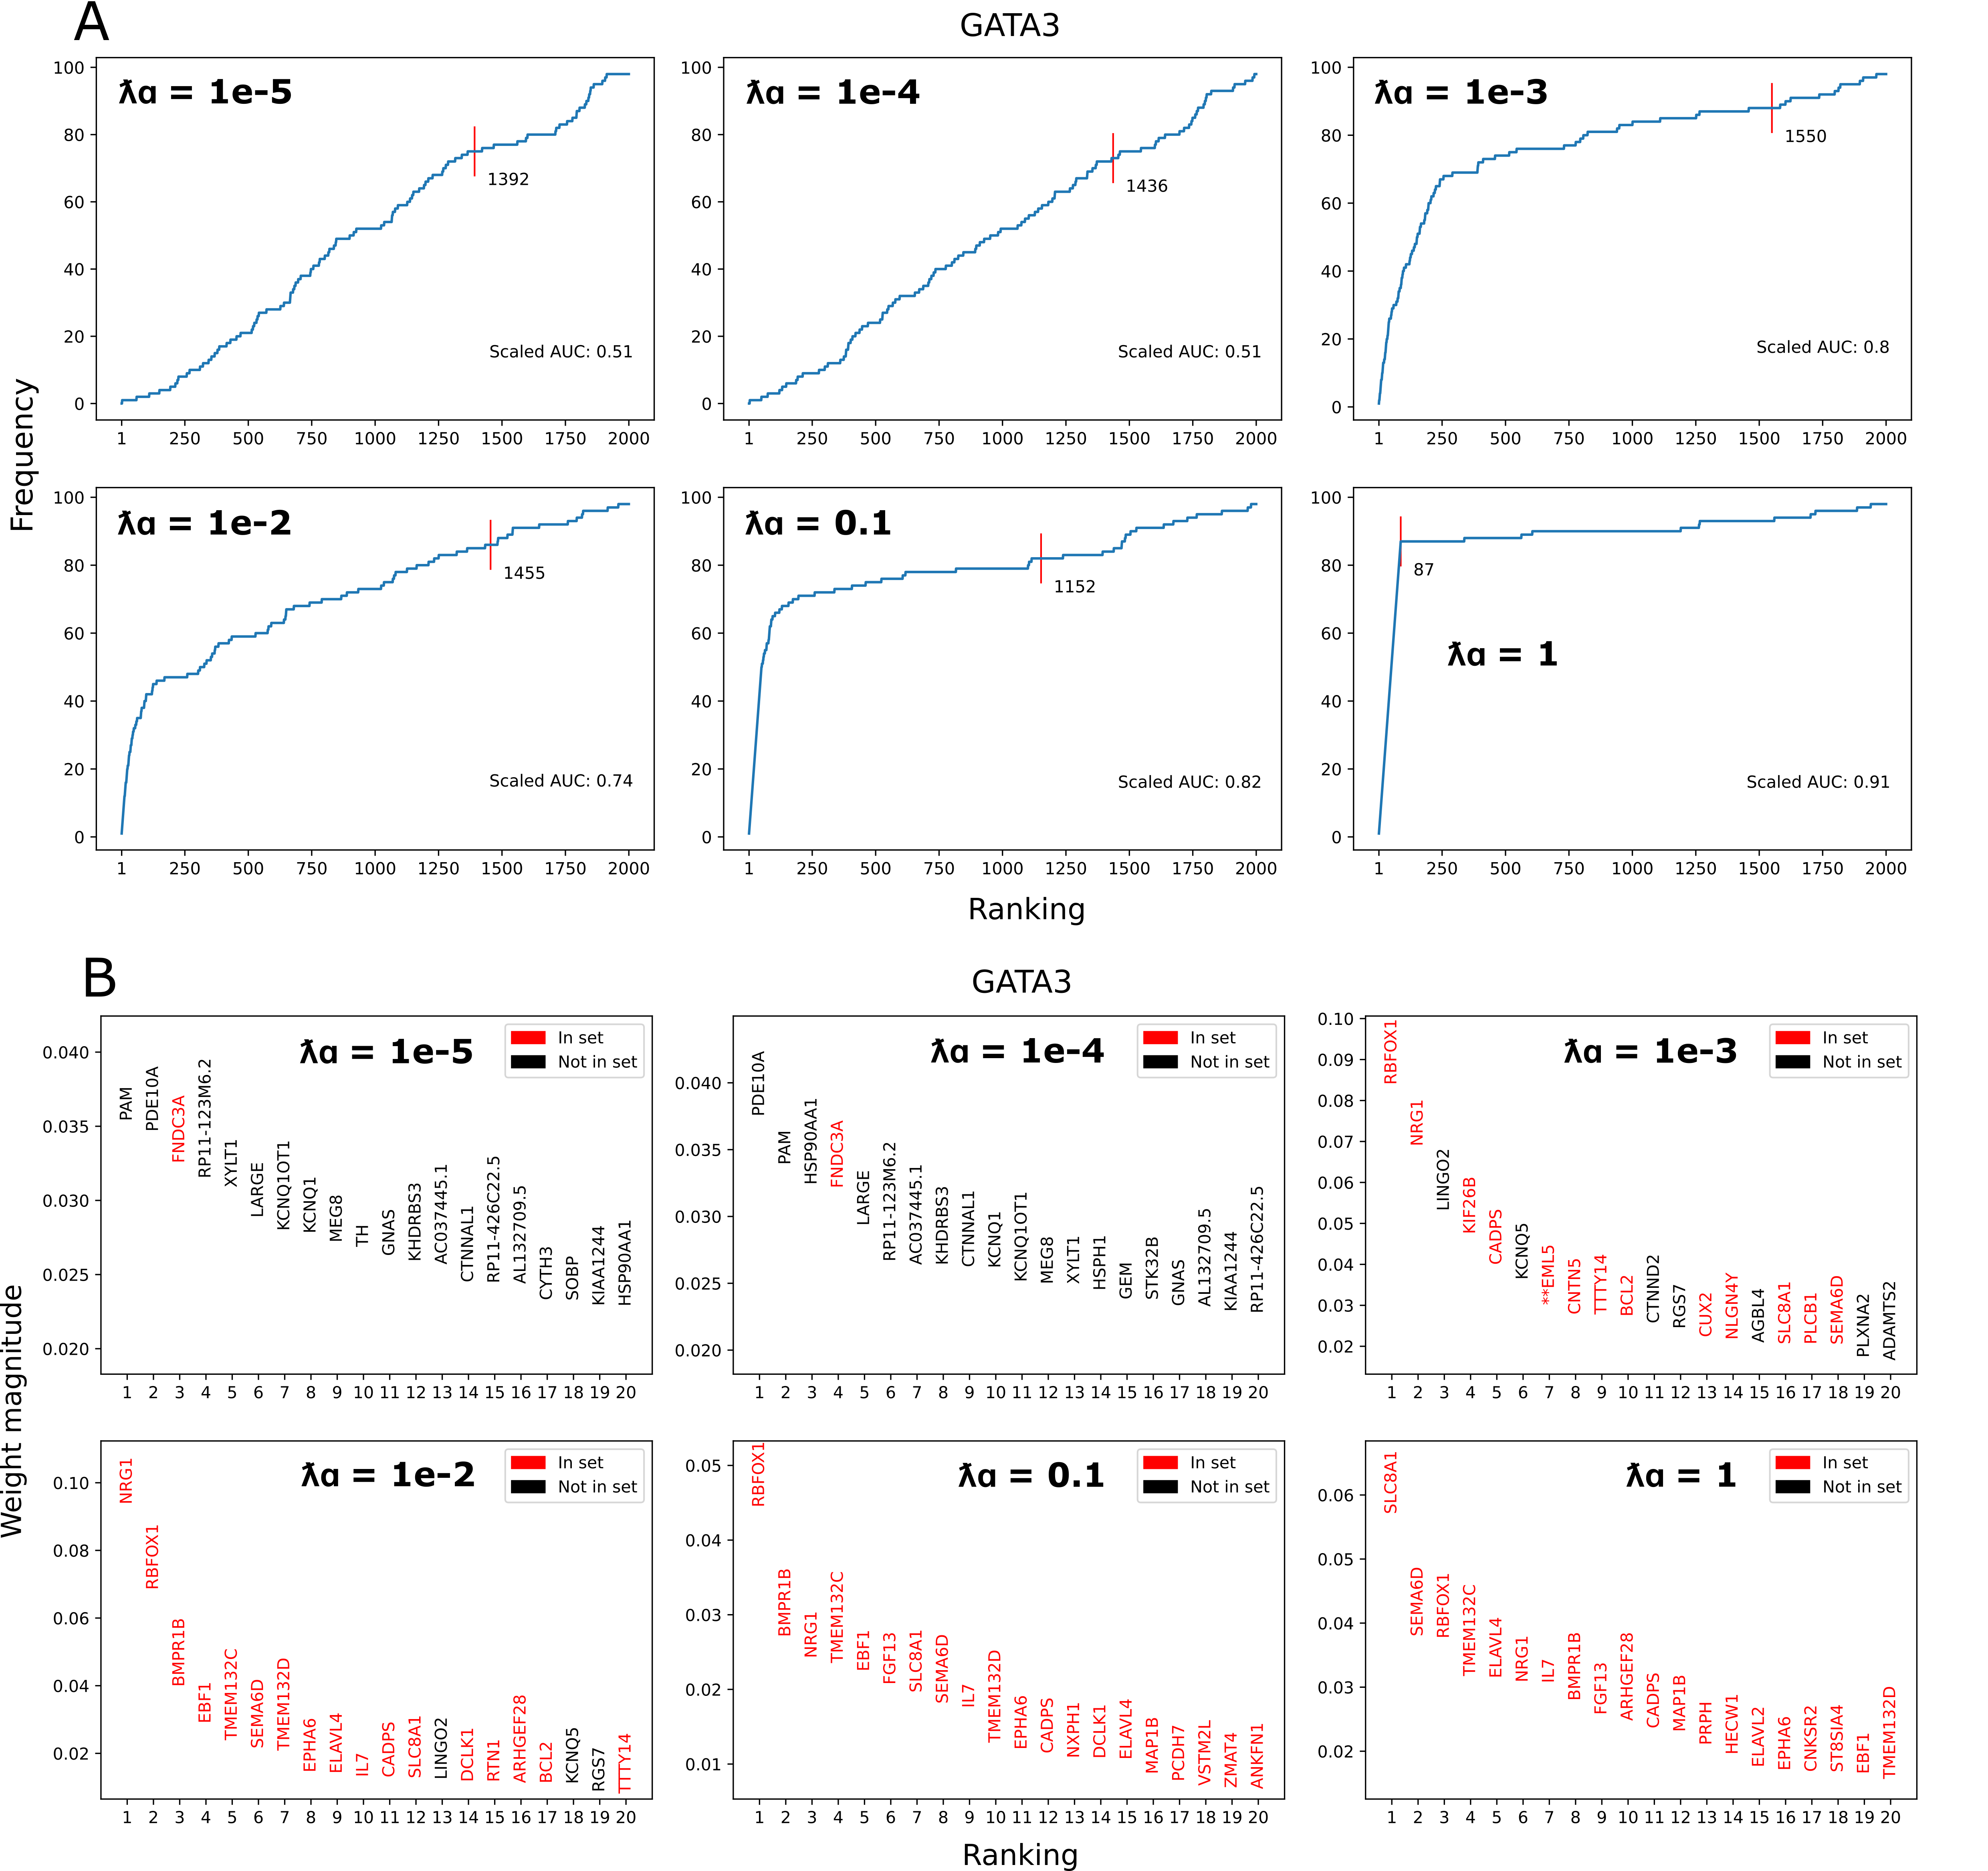
\includegraphics[scale=0.72]{SCENIC_L1/adm_L1_removal.png}
    \caption{\small{The caption is on the previous page.}}
    \label{fig:L1_adm_removal}
\end{figure}

\newpage

\begin{table}[h!]
    \begin{center}
        \captionsetup{width=.76\textwidth}
        \caption{\small{\textbf{Rankings of artificially removed genes} | \textit{EML5}, \textit{STMN2} and \textit{ALK} were artificially removed from the SCENIC GATA3 regulon and \textit{DDC}, \textit{ROBO1} and \textit{GRK5} were artificially removed from the SCENIC JUN regulon. NA indicates that the weight of GATA3 or JUN to the certain gene reconstruction was zero, which means the artificially removed gene was not recovered.}}
        \label{table:L1_removal_ranking}
        \begin{tabular}{|c|c|c|c|c|c|c|}
        \hline
        & \small{GATA3} & & & \small{JUN} & &\\
        & \small{\textit{\textbf{EML5}}} & \small{\textit{\textbf{STMN2}}} & \small{\textit{\textbf{ALK}}} & \small{\textit{\textbf{DDC}}} & \small{\textit{\textbf{ROBO1}}} & \small{\textit{\textbf{GRK5}}}\\
        \hline
        \small{\boldmath{$\lambda\alpha = 10^{-5}$}} & \small{838} & \small{NA} & \small{110} & \small{22} & \small{773} & \small{6}\\
        \hline
        \small{\boldmath{$\lambda\alpha = 10^{-4}$}} & \small{1430} & \small{NA} & \small{121} & \small{293} & \small{NA} & \small{138}\\
        \hline
        \small{\boldmath{$\lambda\alpha = 10^{-3}$}} & \textbf{7} & \textbf{29} & \textbf{32} & \textbf{114} & \textbf{102} & \textbf{105}\\
        \hline
        \small{\boldmath{$\lambda\alpha = 10^{-2}$}} & \small{77} & \small{55} & \small{59} & \small{118} & \small{738} & \small{126}\\
        \hline
        \small{\boldmath{$\lambda\alpha = 0.1$}} & \small{81} & \small{64} & \small{80} & \small{155} & \small{NA} & \small{169}\\
        \hline
        \small{\boldmath{$\lambda\alpha = 1$}} & \small{NA} & \small{NA} & \small{NA} & \small{NA} & \small{NA} & \small{NA}\\
        \hline
        \end{tabular}
    \end{center}
\end{table}

\subsection{Model excludes artificially added genes}\label{sec:L1_adm_added}
Secondly, we investigated how the model using the L1 regularized decoder treats artificially added genes in prior knowledge using the same human adrenal medulla dataset\cite{Jansky2021} and the same strategy described in Section \ref{sec:L1_adm_removed}. Since we observed that the regularized decoder tends to capture genes whose expression levels are averagely high for regulon inferences, i.e., a large proportion of high-ranking putative target genes of a TF have high average expression levels in the single-cell transcriptome data, e.g., GATA3 (Fig.\ref{fig:L1_adm_removal}B), we were inspired to study the behavior of the regularized decoder in two aspects: Artificially adding genes with either high average expression levels or low average expression levels. The way we selected added genes was computing the mean of expression values of each gene across all cells, ranking the genes based on the average expression levels and avoiding picked genes being biologically meaningful to a certain regulon by looked over a couple of existing databases, such as DoRothEA\cite{Garcia-Alonso2019}, Harmonizome\cite{Rouillard2016}, KnockTF\cite{Feng2020}, etc. For instance, we artificially added three genes with high expression levels: \textit{GNAS}, \textit{MEG8} and \textit{NRXN1} and three genes with low expression levels: \textit{PRDM16}, \textit{MEGF6} and \textit{AJAP1} into the SCENIC GATA3 regulons in the duplicate files containing the prior to create two versions of modified prior knowledge. We then systematically trained several individual models using different $\lambda\alpha$ values and these two versions of artificially modified prior knowledge and checked the rankings of weights of the artificially added non-biologically meaningful genes. The hyperparameters used in this task can be found in Appendix \ref{appendixA}. Notice that the behavior of the regularized decoder using different $\lambda\alpha$ values is very similar to our previous findings that the regularized decoder behaves in a more fully-connected way when $\lambda\alpha < 10^{-3}$, in a regularized way when $10^{-3} \leq \lambda\alpha < 1$ and in a hard-coded way when $\lambda\alpha = 1$ (Appx.\ref{fig:L1_adm_addition_appx}). The results show that, when $\lambda\alpha = 10^{-5}$ and $10^{-4}$, the artificially added genes with high expression levels had the higher average rankings than the added genes with low expression levels, which is in line with our previous observations that the decoder tends to capture genes with high average expression levels (Table \ref{table:L1_addition_ranking_GATA3}). Theoretically, the reason might be that genes with high average expression levels usually indicates that genes also have high variances, which might need larger weights to take care of more variable gene reconstructions in the decoder. When $10^{-3} \leq \lambda\alpha < 1$ where the regularized decoder uses the prior evidently, some of the artificially added genes could be excluded, yet the changes in the rankings across different $\lambda\alpha$ values did not have a clear pattern (Table \ref{table:L1_addition_ranking_GATA3}). Roughly, the regularized decoder could best exclude the artificially added genes with high and low expression levels when $\lambda\alpha = 0.1$. Interestingly, when $\lambda\alpha = 1$, all of the artificially added genes with low expression levels were excluded while the added genes with high expression levels were kept, which corroborates again that genes with high expression levels (high variances) are more likely to be captured by the decoder (Table \ref{table:L1_addition_ranking_GATA3}).

Similarly, apart from GATA3, we performed the same analyses on another TF, JUN. We artificially added three genes with high expression levels: \textit{RBFOX1}, \textit{MEG8} and \textit{DLGAP1} and three genes with low expression levels: \textit{PRDM16}, \textit{TSHR} and \textit{PTPRT} into the SCENIC JUN regulons in the duplicate files containing the prior information. At first glance, the ranking results of these added genes from JUN are not very similar to those from GATA3. When $\lambda\alpha = 10^{-5}$ and $10^{-4}$, there was no obvious contrast between the rankings of the artificially added genes with high expression levels and those with low expression levels and, interestingly, \textit{RBFOX1} whose expression level is averagely high was not captured by the decoder, which is not in line with our earlier hypothesis and finding in the example of GATA3 (Table \ref{table:L1_addition_ranking_JUN}). When $10^{-3} \leq \lambda\alpha < 1$, in general, the artificially added genes acquired higher rankings when $\lambda\alpha$ increased and the regularized decoder seemed to be able to exclude the added genes with low expression levels when $\lambda\alpha$ was set to $10^{-2}$ (Table \ref{table:L1_addition_ranking_JUN}). When $\lambda\alpha = 1$, all of the artificially added genes were kept except \textit{PRDM16} and the added genes with high expression levels had the higher average ranking than those with low expression levels (Table \ref{table:L1_addition_ranking_JUN}). Collectively, the regularized decoder has the potential to exclude artificially added non-biologically meaningful genes, yet there is no specific pattern on how the regularized decoder behaves with different values of $\lambda\alpha$. Therefore, further work on how to generalize this technique to all genes is needed.

\begin{table}[h!]
    \begin{center}
        \captionsetup{width=.83\textwidth}
        \caption{\small{\textbf{Rankings of artificially added genes in SCENIC GATA3 regulon} | We split the task into two parts: artificially adding the genes with high average expression levels (\textit{GNAS}, \textit{MEG8} and \textit{NRXN1}) and the genes with low average expression levels (\textit{PRDM16}, \textit{MEGF6} and \textit{AJAP1}) into the SCENIC GATA3 regulons in the duplicate files containing the prior. The rankings marked in bold represent relatively better outcomes of our testing. NA indicates that the weight of GATA3 to the certain gene reconstruction was zero, which means the artificially added gene was not included in the putative GATA3 regulon.}}
        \label{table:L1_addition_ranking_GATA3}
        \begin{tabular}{|c|c|c|c|c|c|c|}
        \hline
        & \small{HIGH} & & & \small{LOW} & &\\
        & \small{\textit{\textbf{GNAS}}} & \small{\textit{\textbf{MEG8}}} & \small{\textit{\textbf{NRXN1}}} & \small{\textit{\textbf{PRDM16}}} & \small{\textit{\textbf{MEGF6}}} & \small{\textit{\textbf{AJAP1}}}\\
        \hline
        \small{\boldmath{$\lambda\alpha = 10^{-5}$}} & \small{17} & \small{12} & \small{724} & \small{1158} & \small{NA} & \small{196}\\
        \hline
        \small{\boldmath{$\lambda\alpha = 10^{-4}$}} & \small{21} & \small{2} & \small{503} & \small{1024} & \small{303} & \small{NA}\\
        \hline
        \small{\boldmath{$\lambda\alpha = 10^{-3}$}} & \small{71} & \small{NA} & \small{242} & \small{NA} & \small{348} & \small{440}\\
        \hline
        \small{\boldmath{$\lambda\alpha = 10^{-2}$}} & \small{936} & \small{NA} & \small{NA} & \small{NA} & \small{143} & \small{191}\\
        \hline
        \small{\boldmath{$\lambda\alpha = 0.1$}} & \textbf{603} & \textbf{NA} & \textbf{NA} & \textbf{951} & \textbf{NA} & \textbf{166}\\
        \hline
        \small{\boldmath{$\lambda\alpha = 1$}} & \small{35} & \small{14} & \small{94} & \small{NA} & \small{NA} & \small{NA}\\
        \hline
        \end{tabular}
    \end{center}
\end{table}

\begin{table}[h!]
    \begin{center}
        \captionsetup{width=.86\textwidth}
        \caption{\small{\textbf{Rankings of artificially added genes in SCENIC JUN regulon} | We split the task into two parts: artificially adding the genes with high average expression levels (\textit{RBFOX1}, \textit{MEG8} and \textit{DLGAP1}) and the genes with low average expression levels (\textit{PRDM16}, \textit{TSHR} and \textit{PTPRT}) into the SCENIC JUN regulons in the duplicate files containing the prior. The rankings marked in bold represent relatively better outcomes of our testing. NA indicates that the weight of JUN to the certain gene reconstruction was zero, which means the artificially added gene was not included in the putative JUN regulon.}}
        \label{table:L1_addition_ranking_JUN}
        \begin{tabular}{|c|c|c|c|c|c|c|}
        \hline
        & \small{HIGH} & & & \small{LOW} & &\\
        & \small{\textit{\textbf{RBFOX1}}} & \small{\textit{\textbf{MEG8}}} & \small{\textit{\textbf{DLGAP1}}} & \small{\textit{\textbf{PRDM16}}} & \small{\textit{\textbf{TSHR}}} & \small{\textit{\textbf{PTPRT}}}\\
        \hline
        \small{\boldmath{$\lambda\alpha = 10^{-5}$}} & \small{NA} & \small{325} & \small{893} & \small{628} & \small{794} & \small{NA}\\
        \hline
        \small{\boldmath{$\lambda\alpha = 10^{-4}$}} & \small{NA} & \small{663} & \small{590} & \small{708} & \small{1038} & \small{1000}\\
        \hline
        \small{\boldmath{$\lambda\alpha = 10^{-3}$}} & \small{894} & \small{51} & \small{NA} & \small{967} & \small{385} & \small{NA}\\
        \hline
        \small{\boldmath{$\lambda\alpha = 10^{-2}$}} & \small{13} & \small{17} & \small{201} & \textbf{NA} & \textbf{NA} & \textbf{379}\\
        \hline
        \small{\boldmath{$\lambda\alpha = 0.1$}} & \small{4} & \small{8} & \small{110} & \small{544} & \small{114} & \small{115}\\
        \hline
        \small{\boldmath{$\lambda\alpha = 1$}} & \small{6} & \small{1} & \small{53} & \small{NA} & \small{172} & \small{169}\\
        \hline
        \end{tabular}
    \end{center}
\end{table}

\subsection{Model infers dataset-specific GRNs using general regulons as prior}\label{sec:L1_dorothea}
In a real-world scenario, existing resources where we require prior biological knowledge are usually not context-specific, but some of those unannotated genes might play an important role in certain biological processes in certain tissues or cells\cite{Seninge2021}. In the previous tasks, we systematically studied the behavior of the model using the regularized linear decoder when the provided SCENIC regulons were artificially modified. We observed that the model was able to recover the artificially removed target genes and exclude the artificially added non-biologically meaningful genes with certain $\lambda\alpha$ values. We further asked whether the model can infer dataset-specific GRNs in the decoder using general regulons as prior knowledge and provide the biologically meaningful latent space. Similarly to the previous strategy and sticking to the human adrenal medulla dataset\cite{Jansky2021}, we systematically trained several individual models using different $\lambda\alpha$ values and the aforementioned DoRothEA\cite{Garcia-Alonso2019} regulons as the prior. The hyperparameters used in this task can be found in Appendix \ref{appendixA}. Since the decoder behaves in a more fully-connected way when $\lambda\alpha < 10^{-3}$ according to our previous observation, we focused on the values of $\lambda\alpha$ between $10^{-3}$ and 1, which makes the decoder in the regularized and hard-coded modes (Fig.\ref{fig:L1_adm_removal}A). The reason that we included the model whose decoder has no freedom to make further inferences about dataset-specific GRNs (when $\lambda\alpha = 1$) was to provide the control group, the contrast to the regularized decoder. We evaluated the inference capacity of the regularized decoder by making recovery plots on the weights of six TFs of interest (GATA3, ETS1, TFAP2B, JUN, FOS and SOX11) based on the corresponding SCENIC regulons and computing the AUC scores of them (see Methods \ref{methods:recovery}). The regularized decoder is considered having the better inference capacity when the AUC scores of those recovery plots are higher, which indicates the greater number of the high-ranking putative target genes are annotated in the SCENIC regulons. Besides, since the DoRothEA and the SCENIC regulons barely overlap with each other (Table \ref{table:dorothea_scenic_outline}), we also included the recovery curves based on the DoRothEA regulons to investigate how the regularized decoder treats those target genes from the DoRothEA prior. The results show that, in general, the inference performance of the regularized decoder was gradually ameliorated when the values of $\lambda\alpha$ increased (increasing AUC scores), except the inference of the GATA3 regulon, and had the best inference capacity when $\lambda\alpha = 0.9$ (Fig.\ref{fig:L1_adm_dorothea_hvgA}A, blue curves). As expected, when $\lambda\alpha = 1$, the regularized decoder lost its inference capacity because of a hard-coded nature of the decoder (Fig.\ref{fig:L1_adm_dorothea_hvgA}A, blue curves). For the gene regulatory information provided by the DoRothEA regulons, as the regular behavior of the regularized decoder, the prior was used more evidently when the $\lambda\alpha$ values increased, which indicates the model preserved the target genes from the DoRothEA regulons while making the inferences about the SCENIC regulons (Fig.\ref{fig:L1_adm_dorothea_hvgA}A, green curves). Furthermore, to check the interpretability in the latent space, we performed UMAP and differential activity analysis on the embedding of the model using $\lambda\alpha = 0.9$, which had the best inference performance. The UMAP plot shows that the model could well cluster cells into cell types and preserve the developmental trajectories of the adrenal medulla (Fig.\ref{fig:L1_adm_dorothea_hvgBC}B). The volcano plots reveal that the model could capture more cell type-specific differential TF activities compared to the results from VEGA using the DoRothEA regulons as the prior (Fig.\ref{fig:sparse_adm_dorothea_hvg}B), yet some of those significantly differential TF activities were falsely predicted, e.g., CUX1, NFATC1 and NR2F2 (Fig.\ref{fig:L1_adm_dorothea_hvgBC}C). Note that the differential activity analysis results took Fig.\ref{fig:sparse_adm_scenic}C as references. Together, the model has the potential to infer dataset-specific GRNs in the regularized decoder using general regulons as prior knowledge and provide the interpretable context-specific latent space.

Next, to verify the more data-specific regulons inferred by the model were truly based on the DoRothEA regulons, we randomized the DoRothEA gene sets to different degrees (10\%, 50\% and 90\%) to investigate whether the regularized decoder can still keep the inference capacity (see Methods \ref{methods:randomization}). We expected that the regularized decoder should lose its inference capacity when the DoRothEA gene sets are greatly randomized, which indicates the reasonable general regulons as the prior are critical for making inferences about more specific GRNs. Similarly to the description above, the recovery curves based on the SCENIC and the DoRothEA regulons were both included, but we will mainly focus on the observations of the changes in the inference performance of the regularized decoder (blue curves). We first looked into the model with $\lambda\alpha = 0.9$, which had the best inference performance. We observed that, when 10\% and 50\% of the DoRothEA target genes were shuffled, the changes in the inference performance (AUC scores) did not have a clear pattern (Fig.\ref{fig:L1_adm_dorothea_hvgD}D). In some cases, the regularized decoder had the better inference performance when using the randomized DoRothEA gene sets than using the original ones, e.g., GATA3 and in other cases, the better inferences happened when using the 50\% randomized DoRothEA gene sets compared to using the 30\% randomized ones, e.g., TFAP2B. The reason for these results may be that, owing to the low degree of overlapping between the DoRothEA and the SCENIC regulons, some unannotated genes which play an important role in the GRN reconstructions were put into corresponding regulons and some unimportant target genes were removed from regulons during the randomization procedure. Even so, when the DoRothEA target genes were 90\% randomized, nearly all of the GRN inferences, except GATA3, had the low AUC scores which are very similar to the scores obtained from the regularized decoder using the original DoRothEA regulons as prior knowledge when $\lambda\alpha = 1$ (Fig.\ref{fig:L1_adm_dorothea_hvgA}A), which indicates the decoder could not faithfully infer the SCENIC regulons (Fig.\ref{fig:L1_adm_dorothea_hvgD}D). Considering that using $\lambda\alpha = 0.9$ did not give the regularized decoder much freedom to make the inferences, we also looked into the model with $\lambda\alpha = 0.5$ as the sanity check, which had the poorer inference performance than the model with $\lambda\alpha = 0.9$ but still had a tendency to infer the SCENIC regulons. Similarly to the model with $\lambda\alpha = 0.9$, when 10\% and 50\% of the DoRothEA target genes were randomized, the changes in the inference performance did not have an obvious pattern, but when the DoRothEA target genes were 90\% randomized, most of the GRN inferences, except GATA3 and TFAP2B, were lost (Appx.\ref{fig:L1_adm_dorothea_rand_0.5_hvg}). Together, using the reasonable general regulons as prior knowledge is important for the model to make further inferences about more data-specific GRNs in the decoder.

\begin{figure}[b!]
    \caption{\small{\textbf{Context-specific GRN inferences from general prior GRNs} | We trained the model with the regularized decoder on the human adrenal medulla dataset and using the non-context-specific DoRothEA regulons as prior knowledge in an attempt to infer more dataset-specific GRNs. \textbf{(A)} The x-axis indicates the ranking of weights of a certain TF and if the corresponding gene was annotated in the SCENIC regulon (blue curves) or in the DoRothEA regulon (green curves) of the TF, the frequency increased 1 in the y-axis. Note that we will focus on blue curves for investigating the changes in the inference performance of the regularized decoder across different $\lambda\alpha$ values. The columns and the rows of the panel A show the different values of $\lambda\alpha$ and the different TFs. The recovery plots show that the regularized decoder had the best inference performance when $\lambda\alpha = 0.9$ and lost its inference capacity when $\lambda\alpha = 1$ (equivalent to the hard-coded decoder). The red bar on a curve indicates the number of non-zero weights of a certain TF (i.e., the putative regulon of the TF). Note that the zero-valued weights were randomly ranked. \textbf{(B)} The UMAP embedding of the latent space from the model with $\lambda\alpha = 0.9$ shows the clear cell clustering and the developmental trajectories of the adrenal medulla. \textbf{(C)} The x-axis and the y-axis indicate the significance level and the mean absolute difference of GMV activity comparisons between two cell types. The volcano plots reveal that the model using the regularized decoder with $\lambda\alpha = 0.9$ could capture more cell type-specific differential TF activities than using the hard-coded decoder (Fig.\ref{fig:sparse_adm_dorothea_hvg}B), yet there were also slightly more wrongly predicted significantly differential TF activities (colored in green). We considered TFs to be significantly differentially activated when $|\textnormal{log}_e(\textnormal{BF})|>3$. \textbf{(D)} To verify the more dataset-specific regulons were truly inferred from the DoRothEA regulons, we trained the model with $\lambda\alpha = 0.9$ using the prior which was randomized to different levels to investigate the changes in the performance of decoder inferences. The columns and the rows of the panel D show the different TFs and the different degrees of randomization of the prior. The results show that there was no evident pattern of the changes in the inference performance when the prior was 10\% and 50\% randomized and nearly all of the GRN inferences, except GATA3, were lost when the prior was 90\% randomized. Ori indicates the original prior and Rand indicates the degree of randomization of the prior.}}
\end{figure}

\addtocounter{figure}{-1}
\begin{figure}[h!]
    \centering
    \hspace*{-1mm}
    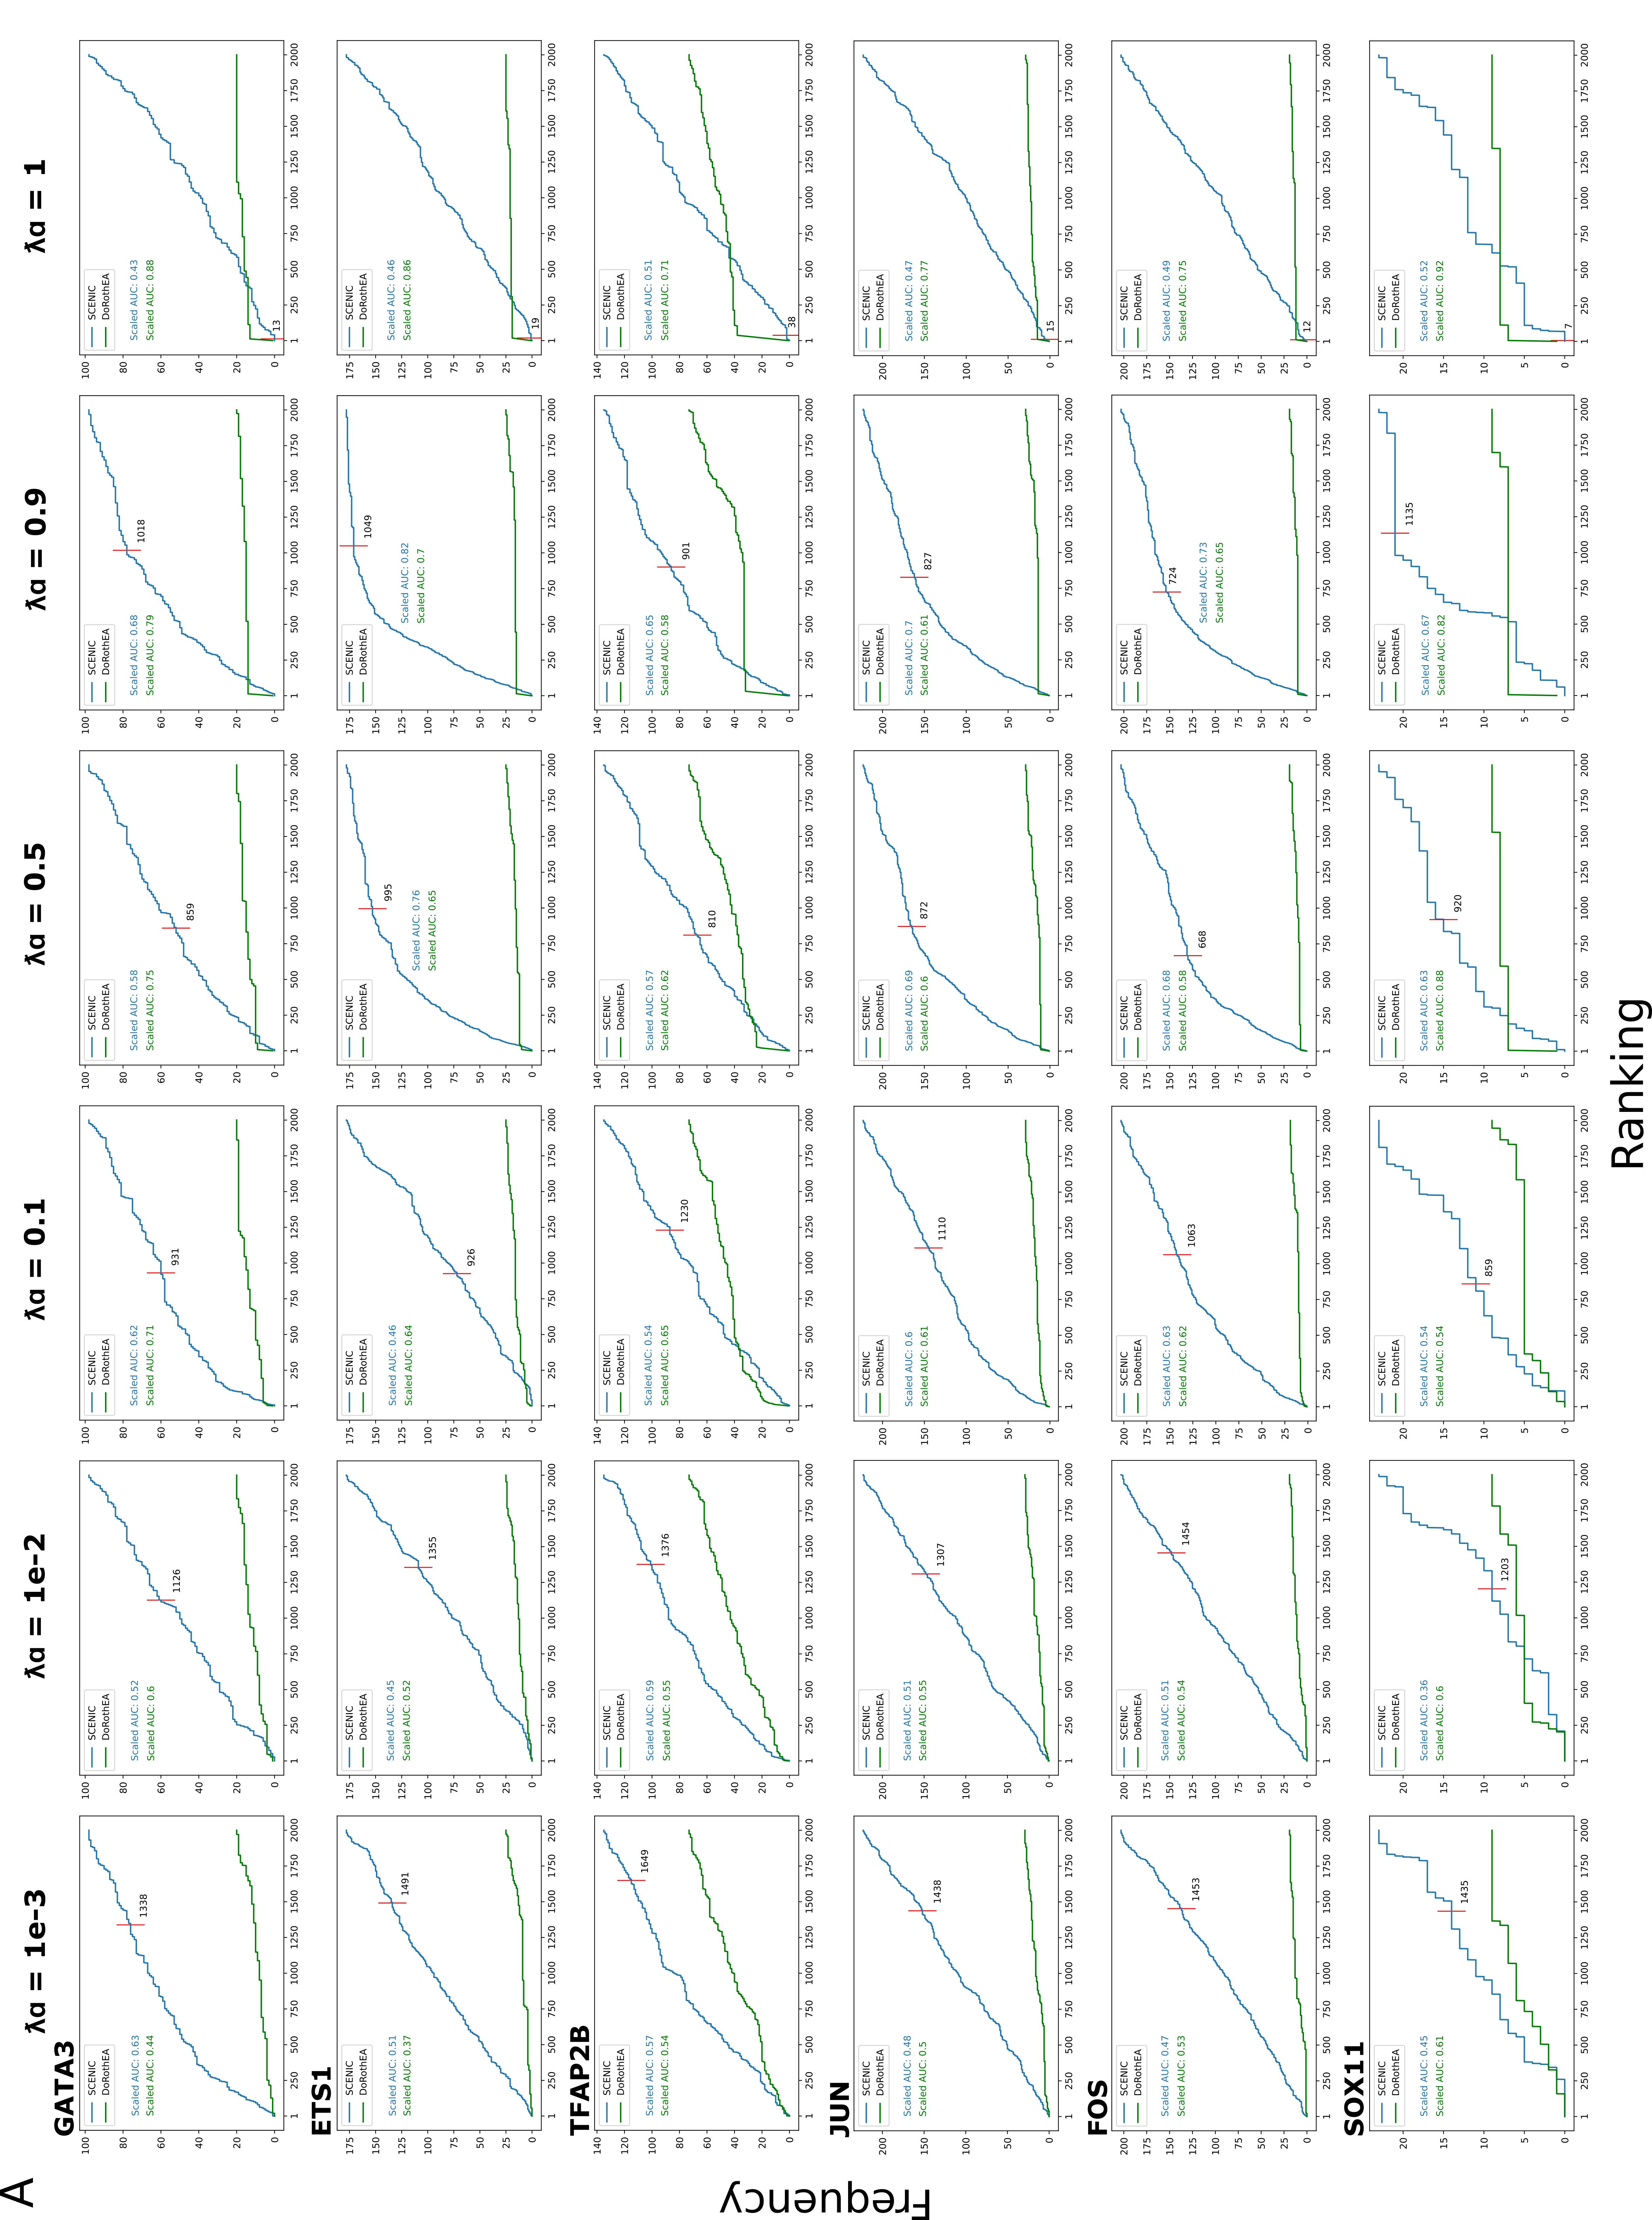
\includegraphics[scale=0.7]{DoRothEA_L1/adm_dorothea_L1_hvg.png}
    \caption{\small{The caption is on the previous page.}}
    \label{fig:L1_adm_dorothea_hvgA}
\end{figure}

\addtocounter{figure}{-1}
\begin{figure}[h!]
    \centering
    \hspace*{-4mm}
    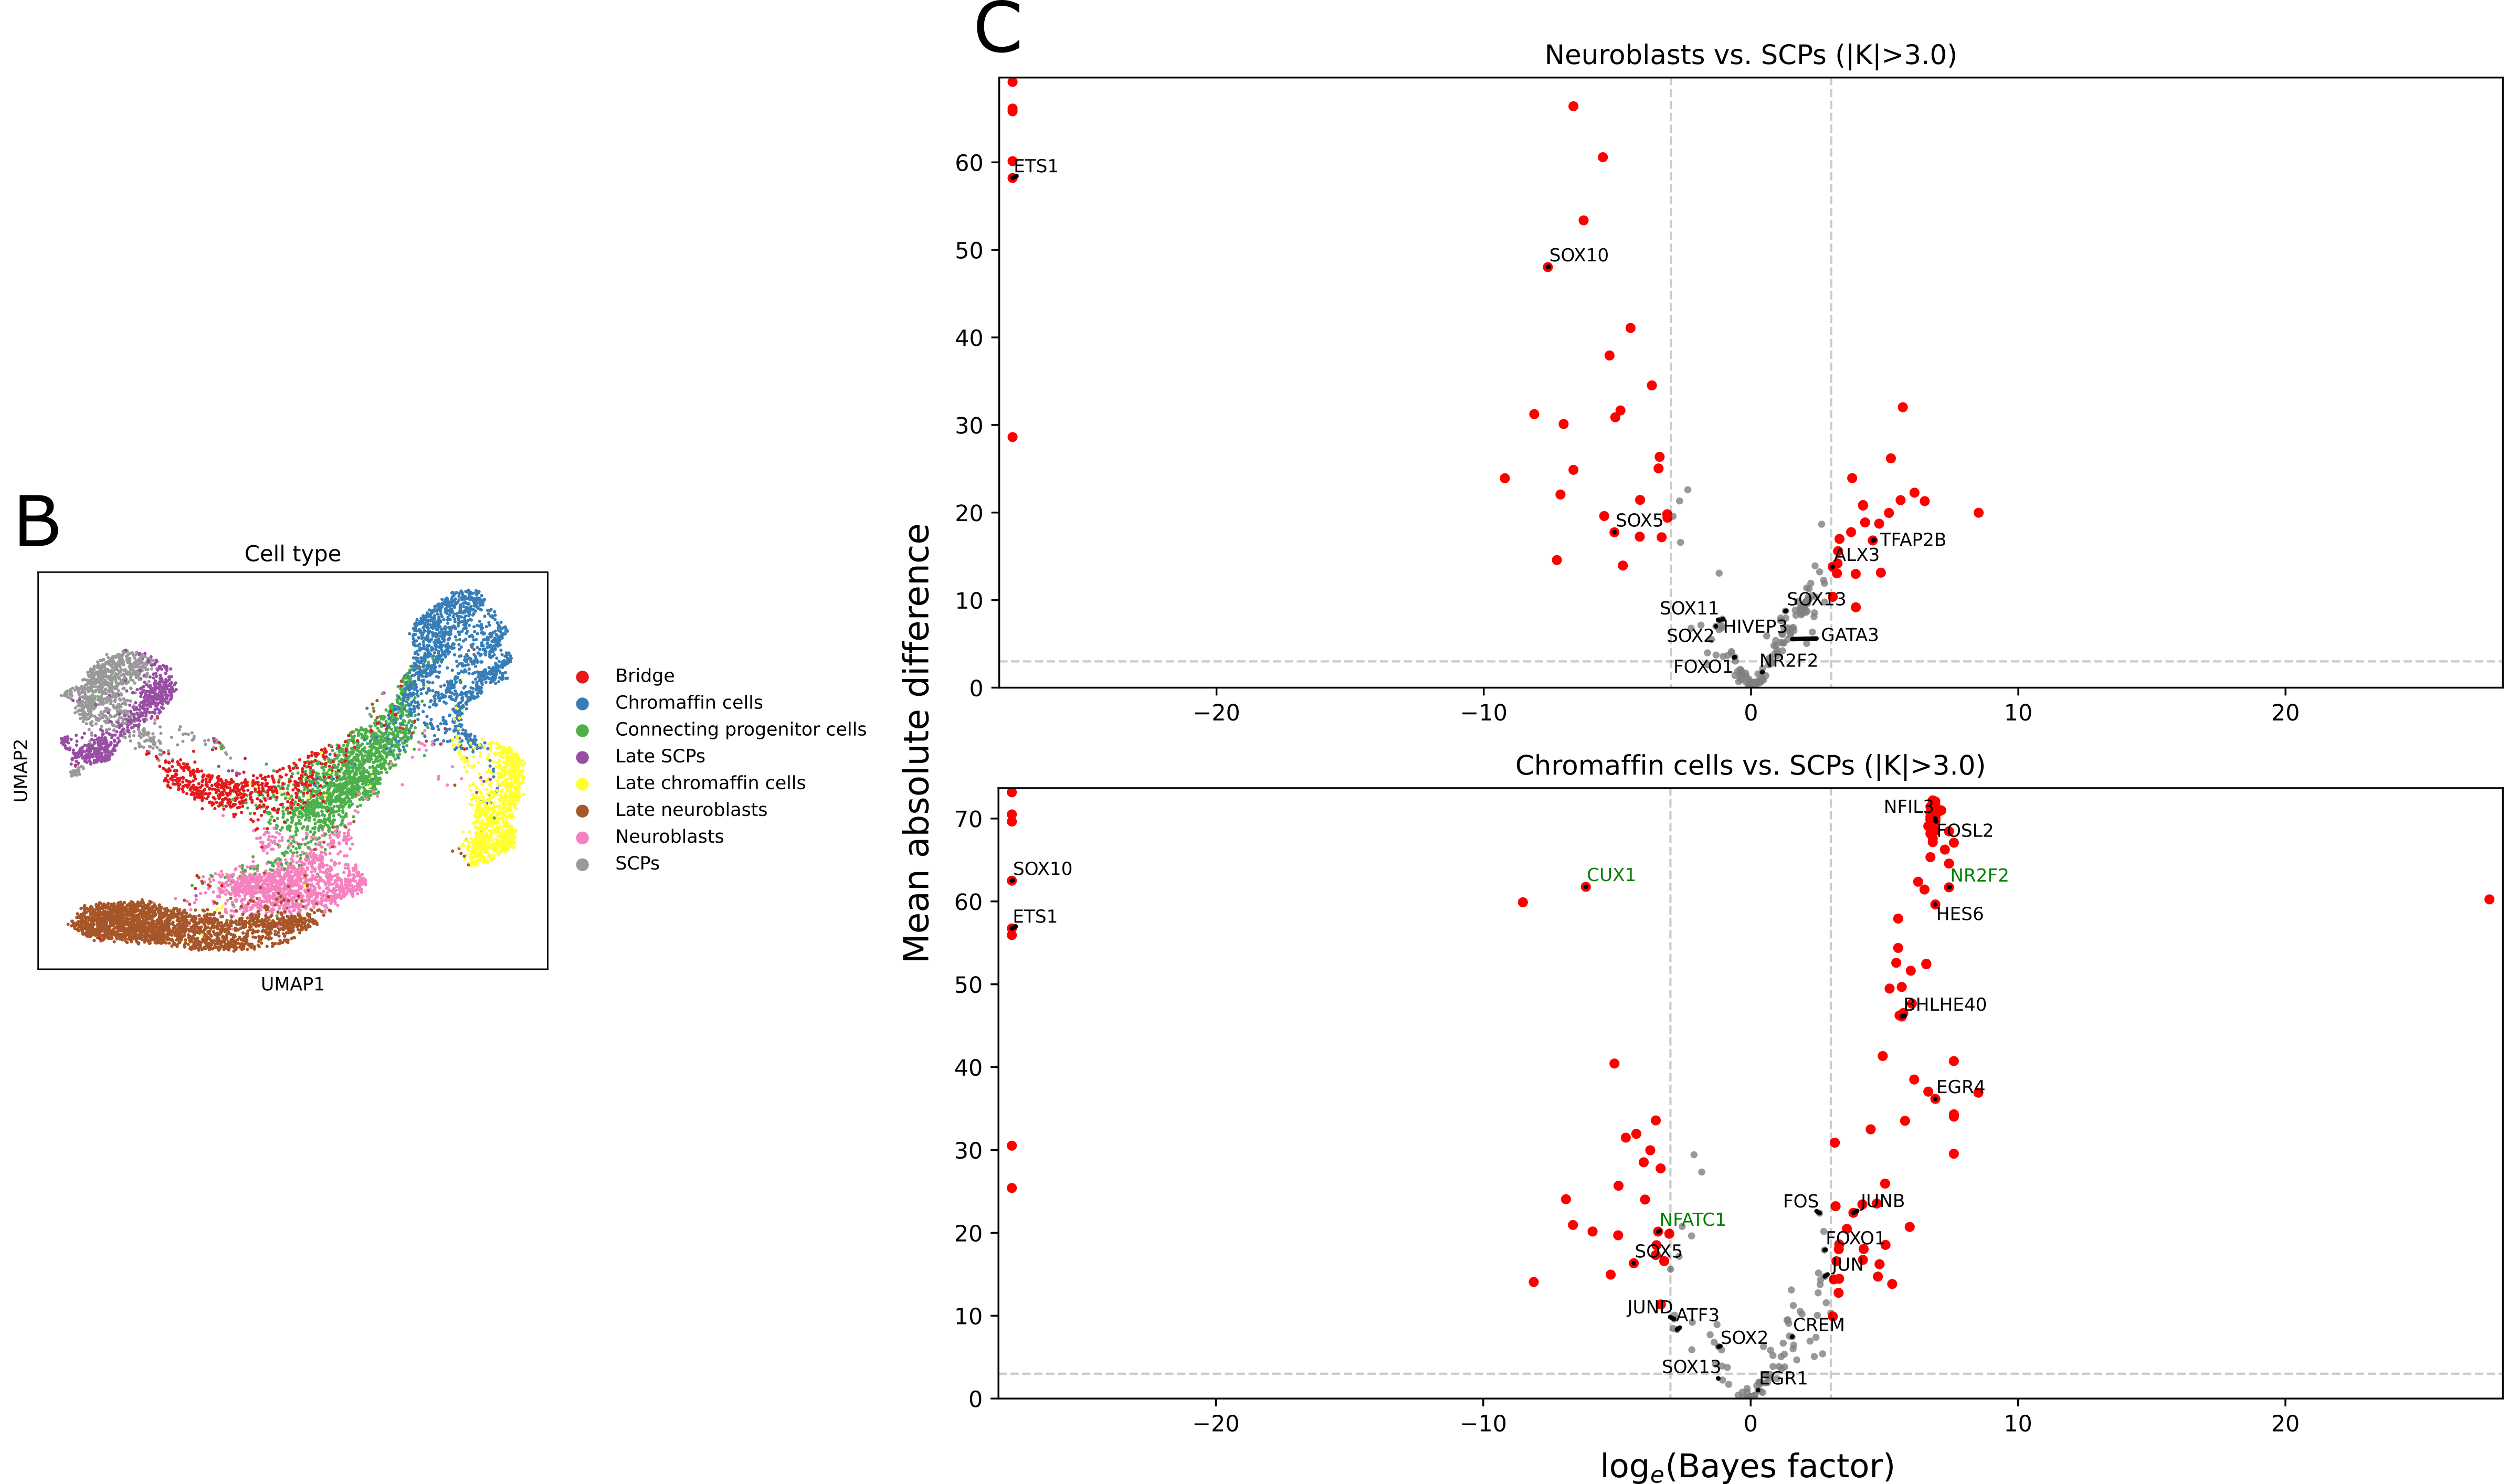
\includegraphics[scale=0.76]{DoRothEA_L1/adm_dorothea_L1_hvg2.png}
    \caption{\small{This figure is continued from the previous page.}}
    \label{fig:L1_adm_dorothea_hvgBC}
\end{figure}

\addtocounter{figure}{-1}
\begin{figure}[h!]
    \centering
    \hspace*{-5mm}
    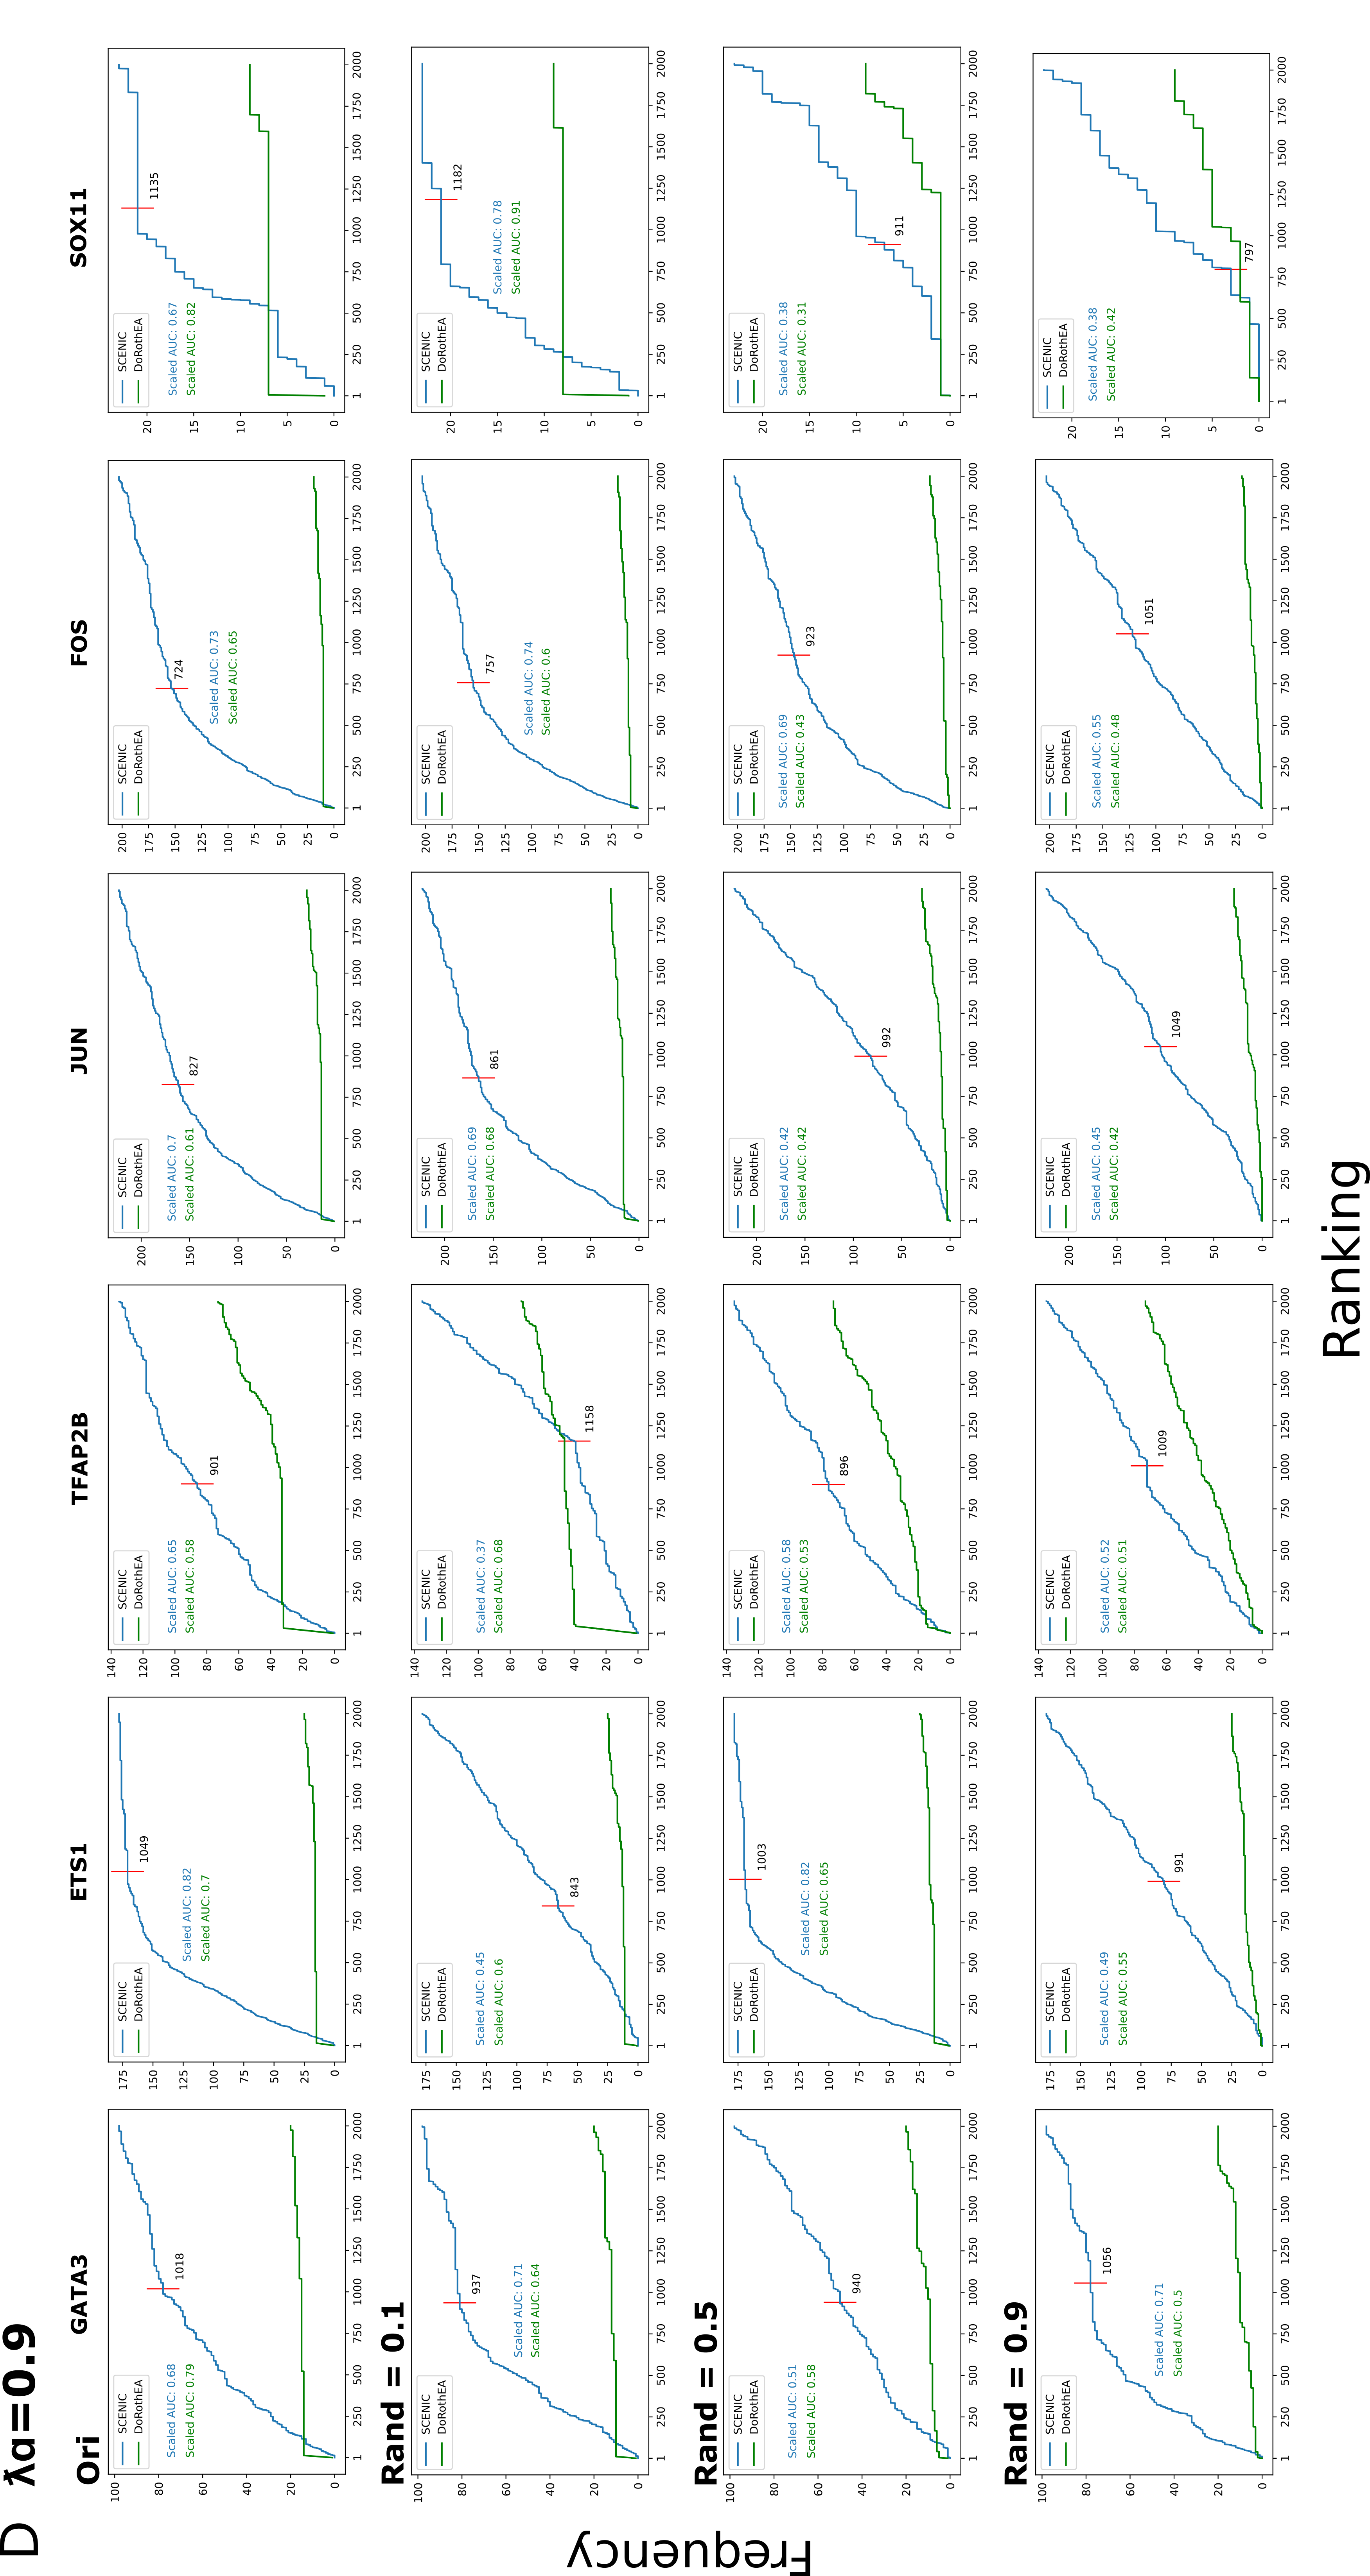
\includegraphics[scale=0.69]{DoRothEA_L1/adm_dorothea_L1_hvg3.png}
    \caption{\small{This figure is continued from the previous page.}}
    \label{fig:L1_adm_dorothea_hvgD}
\end{figure}
